\documentclass[]{elsarticle} %review=doublespace preprint=single 5p=2 column
%%% Begin My package additions %%%%%%%%%%%%%%%%%%%

\usepackage[hyphens]{url}

  \journal{Journal of Hydrology} % Sets Journal name

\usepackage{lineno} % add
  \linenumbers % turns line numbering on

\usepackage{graphicx}
%%%%%%%%%%%%%%%% end my additions to header

\usepackage[T1]{fontenc}
\usepackage{lmodern}
\usepackage{amssymb,amsmath}
\usepackage{ifxetex,ifluatex}
\usepackage{fixltx2e} % provides \textsubscript
% use upquote if available, for straight quotes in verbatim environments
\IfFileExists{upquote.sty}{\usepackage{upquote}}{}
\ifnum 0\ifxetex 1\fi\ifluatex 1\fi=0 % if pdftex
  \usepackage[utf8]{inputenc}
\else % if luatex or xelatex
  \usepackage{fontspec}
  \ifxetex
    \usepackage{xltxtra,xunicode}
  \fi
  \defaultfontfeatures{Mapping=tex-text,Scale=MatchLowercase}
  \newcommand{\euro}{€}
\fi
% use microtype if available
\IfFileExists{microtype.sty}{\usepackage{microtype}}{}
\usepackage[]{natbib}
\bibliographystyle{plainnat}

\ifxetex
  \usepackage[setpagesize=false, % page size defined by xetex
              unicode=false, % unicode breaks when used with xetex
              xetex]{hyperref}
\else
  \usepackage[unicode=true]{hyperref}
\fi
\hypersetup{breaklinks=true,
            bookmarks=true,
            pdfauthor={},
            pdftitle={Generalizing the impact of forest cover on streamflow from experimental data: it is not that simple.},
            colorlinks=false,
            urlcolor=blue,
            linkcolor=magenta,
            pdfborder={0 0 0}}

\setcounter{secnumdepth}{5}
% Pandoc toggle for numbering sections (defaults to be off)


% tightlist command for lists without linebreak
\providecommand{\tightlist}{%
  \setlength{\itemsep}{0pt}\setlength{\parskip}{0pt}}

% From pandoc table feature
\usepackage{longtable,booktabs,array}
\usepackage{calc} % for calculating minipage widths
% Correct order of tables after \paragraph or \subparagraph
\usepackage{etoolbox}
\makeatletter
\patchcmd\longtable{\par}{\if@noskipsec\mbox{}\fi\par}{}{}
\makeatother
% Allow footnotes in longtable head/foot
\IfFileExists{footnotehyper.sty}{\usepackage{footnotehyper}}{\usepackage{footnote}}
\makesavenoteenv{longtable}


\usepackage{setspace}\doublespacing



\begin{document}


\begin{frontmatter}

  \title{Generalizing the impact of forest cover on streamflow from experimental data: it is not that simple.}
    \author[a,b]{R. Willem Vervoort}
   \ead{willem.vervoort@sydney.edu.au} 
    \author[c]{Eliana Nervi}
   \ead{eliananervif@gmail.com} 
    \author[d]{Jimena Alonso}
   \ead{jalonso@fing.edu.uy} 
      \affiliation[a]{Sydney Institute of Agriculture and School of Life and Environmental Sciences, The University of Sydney, Sydney, NSW 2006, Australia}
    \affiliation[b]{ARC ITTC in Data Analytics for Resources and Environments, The University of Sydney, NSW 2006, Sydney, Australia}
    \affiliation[c]{Project Manager, FPTA 358, Instituto Nacional de Investigacion Agropecuaria, INIA-Uruguay, Ruta 48 km 10, Rincon del Colorado, 90100 Canelones, Uruguay}
    \affiliation[d]{Institute of Fluid Mechanics and Environmental Engineering, School of Engineering, Universidad de la Republica, 11200 Montevideo, Uruguay}
    \cortext[cor1]{Corresponding author}
  
  \begin{abstract}
  Three recent papers review and analyze large global datasets related to impacts of forest cover on streamflow. Using three different approaches, they all find a strong relationship between forestation, de-forestation and streamflow. However, the results are problematic, the underlying data set is unbalanced, and there are correlations in the data that warrant further investigation as this would influence the results. For example, the area of the catchment is strongly related to the assessment technique and the variability in the response data. For this study, the data for the recent three papers were reviewed, combined, and supplemented with new studies. Subsequently, the data were re-analyzed using generalized additive modelling.
  The results highlight that there are four interlinked reasons that make the general outcomes from the previous papers problematic: 1) The existence of latent variables in the data that create the appearance of a relationship that really does not exist; 2) The difficulty in fully interpreting the specifics of different studies; 3) The difficulty of integrating data from seemingly similar studies, but with quite different objectives; and 4) The chance of transcription errors influencing the data. Overall this indicates that while valuable data can be extracted from past studies, the above problems need to be considered before results are generalized and extrapolated to continental and global scales.
  \end{abstract}
    \begin{keyword}
    meta analysis \sep forest cover change \sep global scales \sep 
    statistical modelling
  \end{keyword}
  
 \end{frontmatter}

\hypertarget{introduction}{%
\section{Introduction}\label{introduction}}

There is a urgent need to identify the impacts of human intervention on stream flow at a global scale and to separate this from climate effects \citep{wang2020, hoekvandijke2022}. More specifically, the impacts of global deforestation and reforestation are important through their perceived influence on stream flow and blue and green water availability \citep{hoekvandijke2022, schyns2019}. The past work reviewing these impacts \citep{andreassian2004, jackson2005, zhang2017, brown2005, brown2013, filoso2017} highlights a general consensus that if forest areas increase, stream flow decreases and vice-versa. The most dramatic example of this is Figure 5 in \citet{zhang2011} indicating (for Australian catchments) a 100\% decrease in stream flow for catchments with 100\% forest cover. However, on the other end of the spectrum, for three French catchments \citep{cosandey2005}, there was no change in stream flow characteristics in two of the catchments after deforestation. For reforestation, a modelling study across the 1 million km\textsuperscript{2} Murray Darling Basin also found no major effect, especially in larger catchments \citep{vandijk2007}, but a recent study \citep{hoekvandijke2022} found an 8\% change in stream flow as a result of reforestation. Similarly a modelling study by \citet{beck2013} found no significant change in stream flow in 12 catchments in Puerto Rico as a result of deforestation. In contrast, in a recent study in Brazil across 324 catchments, \citet{levy2018} found a significant increase in stream flow, particular in the dry season, as a result of deforestation. This suggests that there can be significant variation across the different studies, methodologies and geographical regions.

For the purpose of this paper, \emph{watershed} and \emph{catchment} are interchangeable terms. Many of the US studies use \emph{watershed}, while European and Australian studies use \emph{catchment}. In particular, we retained the term ``paired watershed studies'' and ``quasi-paired watershed studies'' as this is the most common terminology, but further mostly use the term catchment.

There has been a recent push in the hydrological community \citep{evaristo2020metaanalysis} to use `meta-analysis' to summarize past studies. The suggestion is that, because meta-analyses use clearly defined search terms and statistical methods to analyze the results, this will lead to more reliable summaries of past research. As a result, several review papers have summarized the plethora of forestation and deforestation studies across the globe, in relation to paired watershed studies \citep{brown2005, hewlett1984}, related to reforestation in particular \citep{filoso2017}, and more generally \citep{jackson2005, zhang2017}. These studies aim to generalize the individual experimental and research findings and to identify if there are global trends or relationships. Others have used the understanding from a global analysis to extrapolate to global scales \citep{hoekvandijke2022}.

The recent paper by \citet{filoso2017} is a clear meta-analysis, but most others \citep{zhang2017, hoekvandijke2022, zhou2015} are not. However, n impressive global database of catchment studies with changes in stream flow due to changes in forest cover has been developed \citep{zhang2017, filoso2017} and statistical approaches are used to analyze the resulting data. The \citet{zhang2017} data set, which covers over 312 studies, is described in terms of the change in stream flow as a result of the change in forest cover, where studies related to both forestation (increase in forest cover) and deforestation (decrease in forest cover) were included. In contrast, the paper by \citet{filoso2017} focused primarily on reforestation, and covered an equally impressive database of 167 studies using a systematic review. In this case the collected data is mostly coded as count data and only a subset of 37 studies was analyzed for actual water yield change. There is some overlap between the two data sets, but there are also some studies unique to both sets. The more regionally concentrated and detailed study by \citet{levy2018} is a further independent data set with no overlap with the other studies. However, for this study only the flow and rainfall data is available for the catchments, and the change in land cover was derived from satellite data and was not made available.

The conclusions of the first mentioned major review paper \citep{zhang2017} indicates that there is a distinct difference in the change in flow as a result of forestation or deforestation between small watersheds (catchments), defined as \textless{} 1000 km\textsuperscript{2} and large watersheds (catchments) \textgreater{} 1000 km\textsuperscript{2}. While for small catchments there was no real change in runoff with changes in cover, for large catchments there was a clear trend showing a decrease in runoff with increases in forest cover. The main conclusion was that the response in annual runoff to forest cover was scale dependent and appeared to be more sensitive to forest cover change in water limited catchments relative to energy limited catchments \citep{zhang2017}.

The second study \citep{filoso2017} is a systematic review of reforestation studies (only studies in which forest cover increased). This study classified the historical research and highlighted gaps in the spatial distribution, the types of studies and the types of analysis. Their main conclusion was also that reforestation decreases stream flow, but that there were many interacting factors. For a subset of the data (37 data points) they also indicated decreasing impacts of reforestation with increasing catchment size (agreeing with \citet{zhang2017}), but they did not identify a distinct threshold and fitted a log-linear relationship. In addition, they identified that studies with shorter periods of data collection resulted in larger declines in stream flow.

An earlier paper, that includes much of the same data as \citet{zhang2017} and \citet{filoso2017}, is \citet{zhou2015}, which has one author in common with \citet{zhang2017}. However, this paper aims to explain the variation in the data using the elasticity approach in the Fuh model, which is similar to well-known Budyko approaches \citep{zhang2018elasticity}. In particular, it aims to link the variation in the observed data to variations in the exponent \emph{m} in the Fuh model, which represents vegetation cover. A key observation is that in drier environments, the effects of removing forest cover are much greater than in wetter environments, which is also suggested by Figure 4 in \citet{zhang2017}. The Fuh model and the related variations of the Budyko equilibrium modelling approach was also used by \citet{hoekvandijke2022} to interpret the global impact of reforestation.

However, concerning is that there are some clear limitations in these studies, and some of this applies to meta-analyses in general. The main method in the work by \citet{zhang2017} is a single covariate linear regression. In contrast, the systematic review from \citet{filoso2017} mainly emphasizes the classification and distributions of the study. \citet{zhang2017} points out that a main assumption in their work is that the catchment size threshold at 1000 km\textsuperscript{2} is a distinct separation between ``small'' and ``large'' catchments. However, a subset of 37 data points in \citet{filoso2017} (their Figure 9) does not appear to support this, suggesting a continuum. And while the work \citet{filoso2017} provides important insights in study types, analysis types, forest types and broad classification, there is limited quantification of actual impact.

In contrast to the single covariate linear regression in the earlier studies \citep{zhang2017, filoso2017} and the top-down Budyko modelling \citep{zhou2015, hoekvandijke2022}, the regional Brazilian Cerrado study \citep{levy2018} provides an example of an carefully designed statistical approach using mixed effects modelling and Differences-in-Differences modelling focusing specifically on the effect of deforestation. The analysis specifically accounted for differences between catchments and differences due to variations in climate. Not all data sets are however suitable for this kind of in-depth analysis.

Given all these previous reviews and the seemingly clear conclusions about the impact of forest cover change on stream flow, the question is why another review paper on this topic?
There is a real attraction in the concept of statistical analysis of past studies encapsulated in meta-analysis to be able to extrapolate findings to larger scales, and to identify factors across global scales \citep{evaristo2020metaanalysis}.
However, there are also some hidden complications in this that can invalidate results, which this paper aims to highlight. There are four potential errors (or limitations) in such global meta-analyses:

\begin{itemize}
\tightlist
\item
  Impact of latent variables that are not included in the typical single covariate analysis;
\item
  Interpretation errors due to incomplete descriptions of the experiments in the original papers;
\item
  Aggregation of data that originates from different experiments with different objectives across a wide time period, but have similar keywords; and, finally
\item
  Transcription errors in the data, especially if data is collected from other review papers as some of the original papers are difficult to locate.
\end{itemize}

The aim of this paper is to first reanalyze the global data set \citep{zhang2017, filoso2017} using some more detailed statistical modelling and to use this to highlight examples of each of these limitations. This will show how they have influenced the outcomes of the past work, and provide suggestions of how we can overcome these limitations. In addition, by applying more complex statistical models, we will highlight the conclusions that can be drawn from the data. Finally, we will highlight future research needs in the area of forest cover change impact on stream flow.

We are taking advantage of the earlier work by \citet{zhang2017}, \citet{filoso2017} and \citet{zhou2015} and the large database of studies these authors have shared.

\hypertarget{methods}{%
\section{Methods}\label{methods}}

\hypertarget{the-original-data-set}{%
\subsection{The original data set}\label{the-original-data-set}}

As indicated, the starting point of this paper is the data base of studies which were included in \citet{zhang2017} as supplementary material. The columns in this data set are the catchment number, the catchment name, the Area in km\textsuperscript{2}, the annual average precipitation (Pa) in mm, the forest type, hydrological regime, and climate type, the change in forest cover in \% (\(\Delta F\%\)) and the change in stream flow in \% \((\Delta Qf\%)\), the precipitation data type, the assessment technique, and the source of the info, which is a citation. The change in stream flow (\(\Delta Qf\%\)) is based on equation 1 in \citet{zhang2017}.

Several of these columns contain abbreviations to describe the different variables, which are summarized in Table \ref{tab:table1}. These abbreviations will later be used in the models.

\begin{longtable}[]{@{}
  >{\centering\arraybackslash}p{(\columnwidth - 4\tabcolsep) * \real{0.3611}}
  >{\centering\arraybackslash}p{(\columnwidth - 4\tabcolsep) * \real{0.2083}}
  >{\centering\arraybackslash}p{(\columnwidth - 4\tabcolsep) * \real{0.4167}}@{}}
\caption{\label{tab:table1} Summary of abbreviations of factors used in the Zhang et al.~(2017) data set}\tabularnewline
\toprule()
\begin{minipage}[b]{\linewidth}\centering
Factor
\end{minipage} & \begin{minipage}[b]{\linewidth}\centering
Abbreviation
\end{minipage} & \begin{minipage}[b]{\linewidth}\centering
Definition
\end{minipage} \\
\midrule()
\endfirsthead
\toprule()
\begin{minipage}[b]{\linewidth}\centering
Factor
\end{minipage} & \begin{minipage}[b]{\linewidth}\centering
Abbreviation
\end{minipage} & \begin{minipage}[b]{\linewidth}\centering
Definition
\end{minipage} \\
\midrule()
\endhead
forest type & CF & coniferous forest \\
& BF & broadleaf forest \\
& MF & mixed forest \\
hydrological regime & RD & rain dominated \\
& SD & snow dominated \\
climate type & EL & energy limited \\
& WL & water limited \\
& EQ & equitant \\
precipitation data type & OB & observed \\
& SG & spatial gridded \\
& MD & modelled \\
assessment technique & PWE & paired watershed experiment \\
& QPW & quasi-paired watershed
experiment \\
& HM & hydrological modelling \\
& EA & elasticity analysis \\
& SH & statistical modelling and
hydrographs \\
\bottomrule()
\end{longtable}

The paper by \citet{zhang2017} also uses the dryness index, which is the annual rainfall (Pa) divided by the potential or reference evapotranspiration (ET\textsubscript{0} or E\textsubscript{0}) in their analysis, and have used the dryness index to identify the climate type. However, the potential or reference ET used for this calculation was originally not included in the published data set. We will discus below how we derived the dryness index in our data set. We combined the tables for small catchments (\textless{} 1000 km\textsuperscript{2}) and large catchments (\textgreater= 1000 km\textsuperscript{2}) from \citet{zhang2017} in our analysis.

\hypertarget{additional-data-collection}{%
\subsection{Additional data collection}\label{additional-data-collection}}

To enhance the existing data set, this study added additional variables and cross-checked the studies with the data set from \citet{filoso2017}. In particular, we focused on the 37 data points related to the quantitative regression analysis used in \citet{filoso2017}.

In addition, a few additional variables were included to enhance the data set. We added latitude and longitude for the center of the catchment as an approximation of its spatial location. Mostly the data reported by the authors was used, but in some cases the variables had to be approximated from the location of the centre of the catchment using Google Maps\textsuperscript{TM}. In the data set, an additional column has been added to indicate the source of the location data to indicate if this is directly from the paper or elsewhere.

As highlighted, \citet{zhang2017} did not provide values for evapotranspiration in the data base. Using the location information, reference evapotranspiration (E\textsubscript{0}) was extracted from the Global Aridity Index and Potential Evapo-Transpiration (ET\textsubscript{0}) Climate Databasev2 \citep{trabucco2018}, if a value of E\textsubscript{0} was not available from the original papers. For large catchments, this value (and the associated coordinates), similar to annual average rainfall, is only an approximation of the climate at the location.

Similar to \citet{zhang2017}, the Dryness index was calculated from the catchment estimate of reference evapotranspiration and the catchment estimate of annual average rainfall (Pa) as:

\begin{equation}
Dryness = \frac{E_{0}}{Pa} \label{eq:eq1}
\end{equation}

The length of the study can be a variable influencing the change in flow \citep[e.g.][]{jackson2005, filoso2017}, as for example, more mature plantations are thought to have smaller impacts on flow or regrowth might follow a ``Kuczera curve'' \citep{kuczera1987}. It is not clear if this is an effect of increased water use in growth \citep{vertessy2001} or due to changes in interception \citep{stoof2012}. Therefore, the length of the study calculate as the difference between the starting data and completion date of the different studies was extracted from the references provided by \citet{zhang2017}. The length of the study was already included in the data from \citet{filoso2017}, but these were checked against the original publications.

Several additional data points from catchment studies were extracted from \citet{almeida2016}, \citet{ferreto2020}, \citet{iroume2013}, \citet{iroume2006}, \citet{zhang2011}, \citet{zhao2010}, \citet{borg1988}, \citet{thornton2007}, \citet{zhou2010}, \citet{rodriguez2010}, \citet{ruprechtetal1991} and \citet{penaarancibia2012}, and these were checked against the existing studies to prevent overlap. In the citation column in the accompanying data set, the main reference for the calculated change in stream flow was generally used, because sometimes the original study did not provide the quantification of the change in stream flow \citep[i.e.~Table 6 in][]{zhang2011}.

We conducted a thorough review of all the studies mentioned in the data base of \citet{zhang2017} and sourced all the original papers. As a result of this we made several changes to the data base, which are all recorded in Supplementary Data part 1. Overall 36 data points were changed and the most common problem was a change in the sign for the change in forest cover or the change in flow. We assume that these were transcription errors.\\
We also removed one data point from the data set, which corresponds to catchment \#1 (Amazon) in \citet{zhang2017}. This is because the cited reference \citep{roche1981} only relates to 1 and 1.5 ha paired catchment studies in French Guyana, and in which the actual change in forest cover is not recorded. Finally, on review of all the data in \citet{zhang2017} and \citet{filoso2017}, 29 potential duplicates were identified and flagged in the data, and not used in the analysis.

The final column in the improved data base is a ``notes'' column, which we added, but is not further used in the analysis. It gives context to some of the data for future research and highlights some of the discrepancies that we found between the original papers and the data in the tables from \citet{zhang2017}. This will allow future research to scrutinize our input for errors.

\hypertarget{statistical-modelling}{%
\subsection{Statistical modelling}\label{statistical-modelling}}

The aim of the statistical analysis is to highlight the most important variables in the data set that explain the change in flow as a result of changes in forest cover. This first aim is similar to \citet{zhang2017}, but the main difference is that we start off with all variables in the data set in the model. Subsequently the analysis will concentrate on how the individual variables in the data set relate to each other and how latent variables in the data set can be masked and result in relationships that might not really exist. Finally, the analysis will highlight how the results are conditional on the data set.

In the statistical analysis we are not necessarily seeking the best ``predictive'' model, and as such do not perform a traditional variable selection process. Rather, we focus on analyzing the predictor variables in the full model to identify how all the variables explain the variance in the dependent variable.

To estimate how the change in stream flow is affected by the change in forest cover, while considering the effects of the other variables, we applied generalized additive modelling (GAM) \citep{wood2006}.

The general model tested is:

\begin{align}
\Delta Qf \% \sim &~ \Delta \% forest~cover + \notag \\ 
& \sum{X_i} + \sum{s(Z_i)} + \varepsilon \label{eq:eq2}
\end{align}

Here \(X_i\) are factorial variables, while \(Z_i\) are continuous variables. As a first step, the model assumes no direct interactions and that all variables are additive. A further assumption in the model is that all continuous variables \(Z_i\) (such as annual precipitation (Pa)) can have either a linear or a non-linear relationship with \(\Delta Qf \%\). This means that a smooth function \(s()\) can be applied to the \(Z_i\) variables. For the smoothing function we applied thin plate regression splines with an additional shrinkage penalty. The result of this approach is that for high enough smoothing parameters (i.e.~if the data is very ``wiggly'') the smooth term can be shrunk to 0 and thus will be no longer significant \citep{wood2006}. This is done because a highly flexible smooth term could always fit the data, but would not necessarily indicate a relevant relationship. In other words, the approach balances finding a smooth non-linear relationship for the variable against over fitting the data.

The changes in forest cover contain both positive (forestation) and negative values (deforestation). In \citet{zhang2017}, these changes were jointly analyzed, assuming the effect on the change in flow was linear and the effect of removing forest cover was the same as an equivalent addition of forest cover.

However, the impact of an increase in forest cover can be different from the same fractional decrease in forest cover. The question becomes how best to analyze this. One approach would be to allow a different slope and a different intercept for the decreases relative to the increases.
This can be tested by converting all the change in forest cover data to positive values, and an additional binary column (\(sign_{forest cover}\)) can be included indicating whether it was a forest cover increase or decrease. In the model, the parameter for \(sign_{forest cover}\) will indicate the difference in the changes in flow for increases in forest cover compared to decreases in forest cover. The disadvantage of this approach is that the relationship with forest cover becomes discontinuous at the origin (0 change in forest cover).

A second approach is to test the change in forest cover as a non-linear relationship in the GAM model. Because a shrinkage penalty is used, this will also test the non-linear assumption and allows the variable for forest cover to be continuous. The disadvantage of this approach is that the relationship between forest cover and change in flow is less easy to interpret, as the non-linear fit in the GAM has no direct parametric form.
All three approaches are tested in this study.

The overarching test focuses on identifying the change stream flow as a result of a change in forest cover and how this is potentially affected by different other factors (as indicated by the previous research: \citet{zhang2017}; \citet{filoso2017}; \citet{zhou2015}): climate, size of catchment and length of study. In addition to these earlier identified factors, this study also tested for the factors listed in Table \ref{tab:table1}

As an initial approach we tested whether the additional catchments added to the original data from \citet{zhang2017} did not majorly influenced the results (This analysis is in supplementary material part 2). This analysis highlights that the newly added catchment and the changes to the data set create minor differences when repeating the analysis from the original paper. However, this means that the results of the studies are still comparable.

To make all the data and code used for the analysis publicly available, all the final data and analysis for this paper are located on github:\\
\href{https://github.com/WillemVervoort/Forest_and_water/tree/publish}{https://github.com/WillemVervoort/Forest\_and\_water} on the ``publish'' branch.

\hypertarget{results}{%
\section{Results}\label{results}}

\hypertarget{description-of-the-data}{%
\subsection{Description of the data}\label{description-of-the-data}}

The overall data set contains 334 observations of changes in flow, which includes the newly identified data sets and after removing identified duplicate data and lines with missing data. In contrast, the original data set from \citet{zhang2017} contained 312 catchments and the \citet{filoso2017} study used 37 catchments (Table S2 in \citet{filoso2017}). The overall distribution of changes in flow is highly skewed as is the distribution of changes in forest cover and \emph{Area km\textsuperscript{2}}. The values of changes in flow greater than 100\% and smaller than -100\% clearly create long tails in the change in flow distribution. Note also the large number of studies with 100\% forest cover reduction. Clearly visible is also that smaller catchments dominate the database with 42\% of the data from catchments \textless{} 1 km\textsuperscript{2} and 65\% of the data for catchments \textless{} 10 km\textsuperscript{2} (Figure 1). This high skew in some of the data can create difficulties in the statistical modelling and this will be discussed later.



\begin{figure}
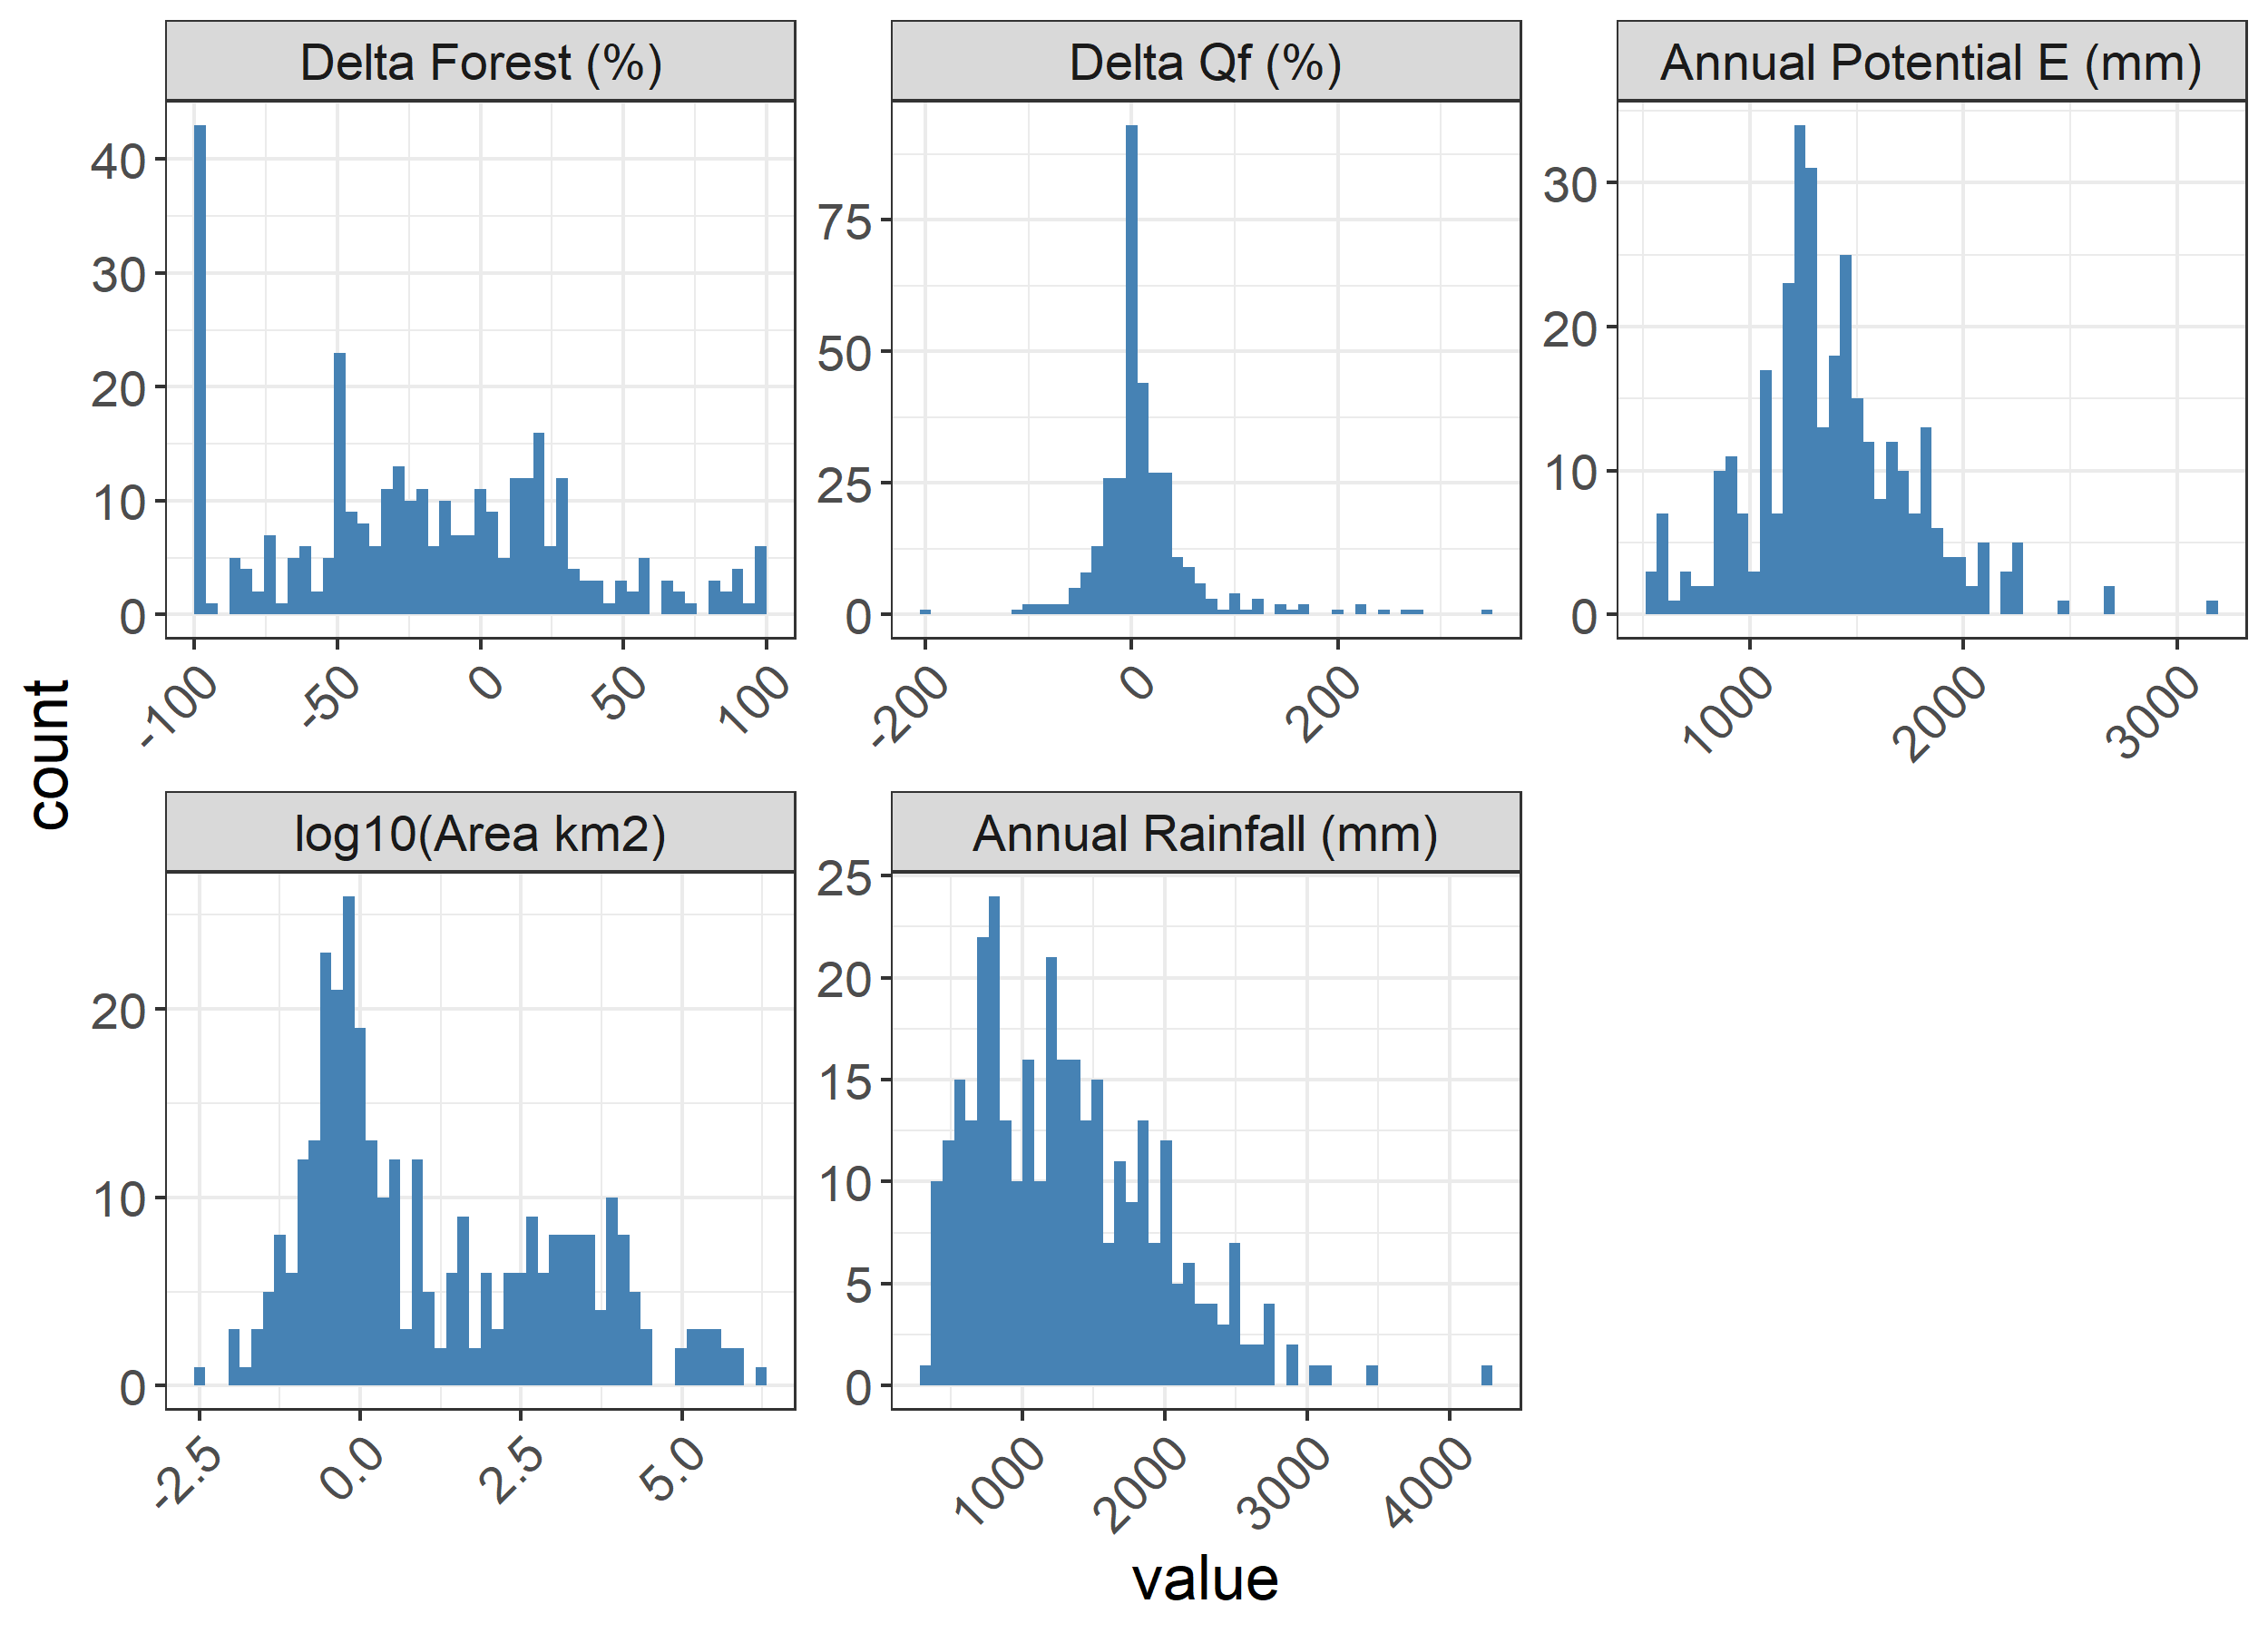
\includegraphics[width=0.9\linewidth]{./DataExploration} \caption{Overview of the distribution of the data set for five of the included variables. Note that the first panel (showing the distribution of the catchment areas) indicates the distribution of the \emph{log\_10\_} transformed Area (in km\textsuperscript{2}).}\label{fig:datagraphs}
\end{figure}

\hypertarget{geospatial-location-of-the-catchments}{%
\subsubsection{Geospatial location of the catchments}\label{geospatial-location-of-the-catchments}}

\begin{figure}
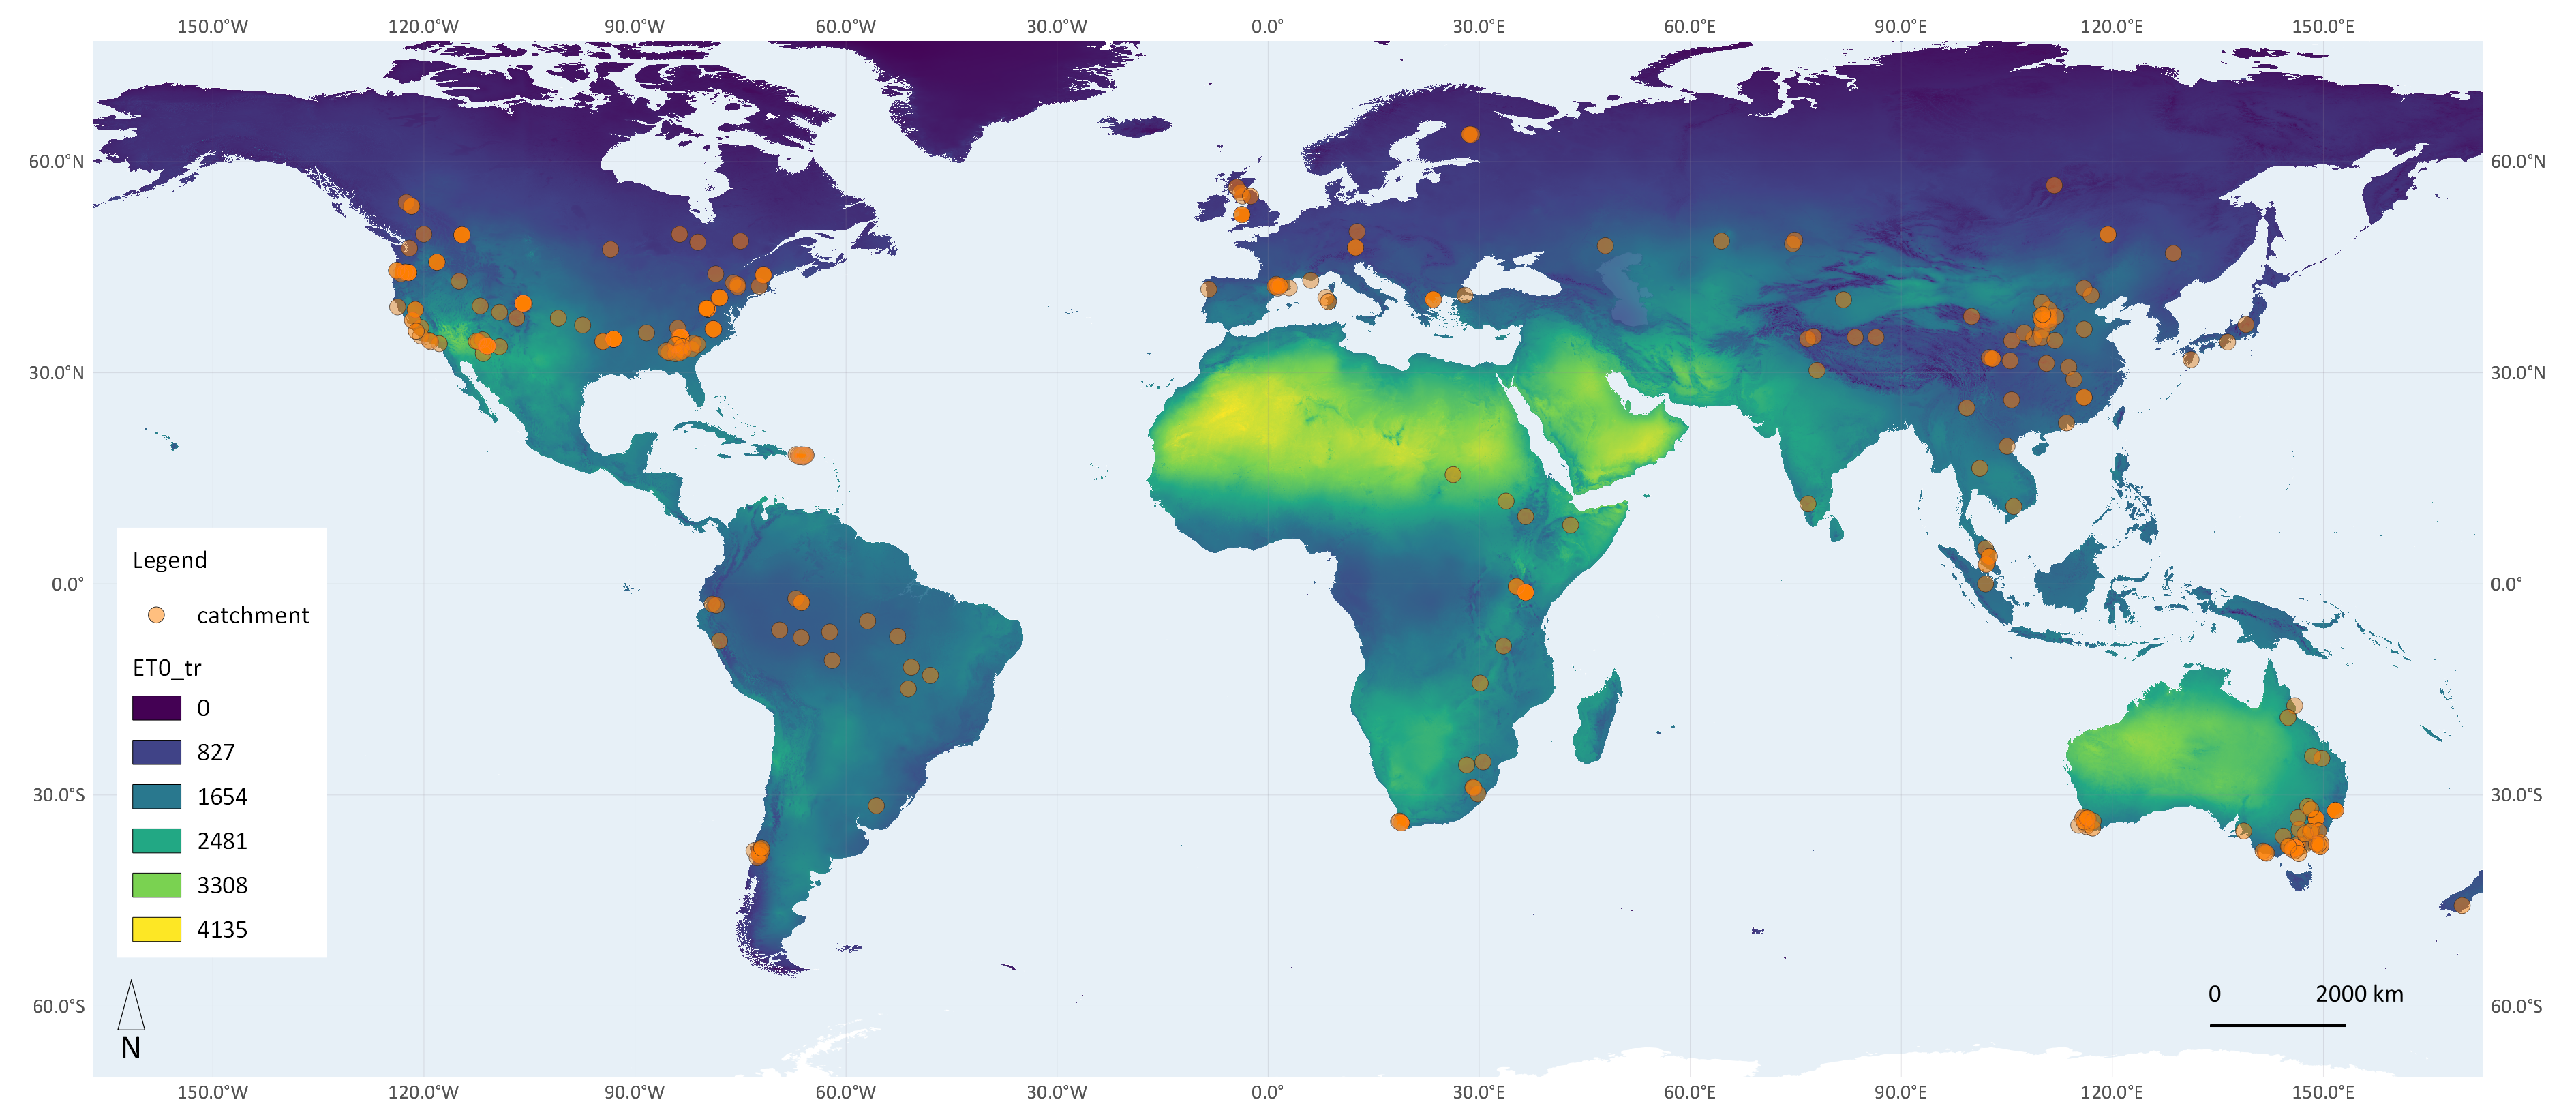
\includegraphics[width=0.9\linewidth]{FAOET0data_final_2022} \caption{Distribution of included catchments across the globe based on reported or estimated latitude and longitude}\label{fig:globalmap}
\end{figure}

Apart from looking at the distribution of the values, the spatial locations of the data can also be important, in particular when analyzing the effect of climate. The catchments are spread across the world, and relative to \citet{zhang2017}, this data set has a very similar geospatial distribution. The major climate gradients are represented in the data, but there appears to be some bias in the spatial locations of the data. As the global map (Figure \ref{fig:globalmap}) shows, the distribution of case study catchments covers multiple continents. There is some spatial clustering in the studies in North America, Australia and East Asia.

\hypertarget{cross-correlation-between-the-different-variables}{%
\subsubsection{Cross correlation between the different variables}\label{cross-correlation-between-the-different-variables}}

A final data exploration is to identify potential cross correlations in the data, which can point to possible interactions or potential biases. This analysis can also provide further insight for the statistical modelling, highlighting potential latent variables in the data set.

\begin{figure}
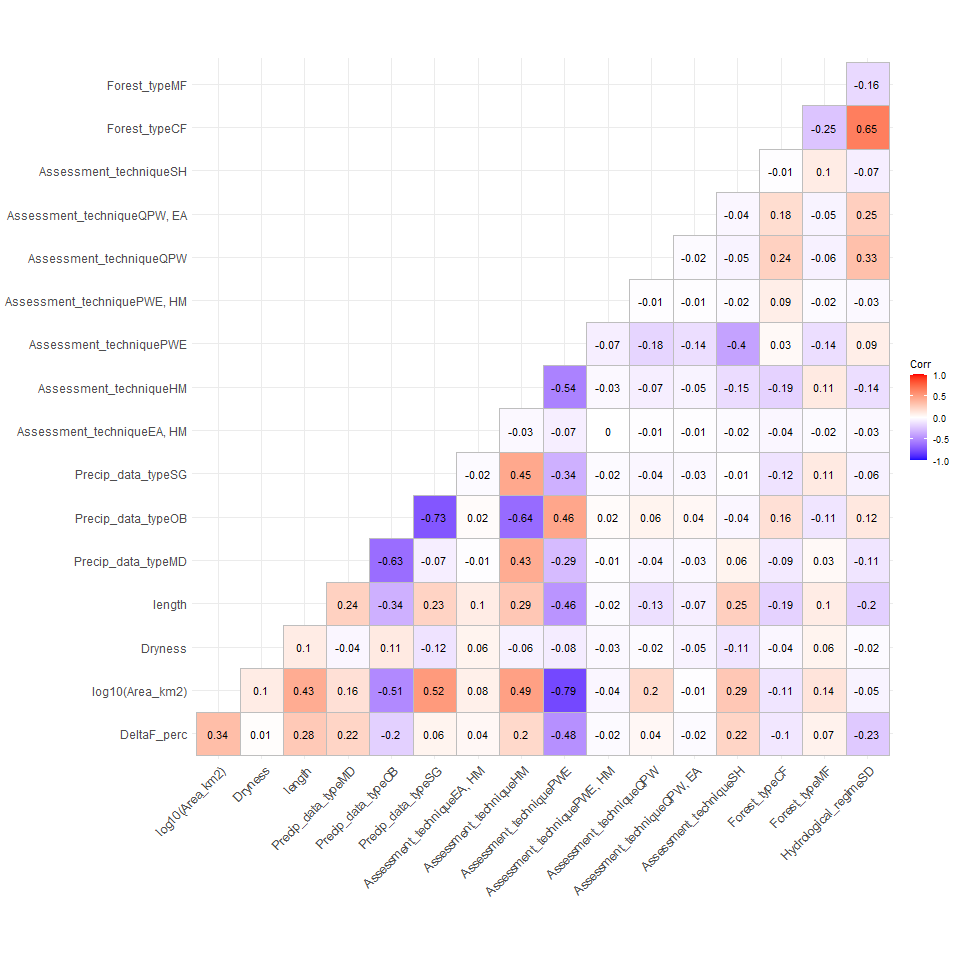
\includegraphics[width=0.9\linewidth]{variable_corr_plot} \caption{Correlation matrix for all variables}\label{fig:corgraphs}
\end{figure}

The correlation plot (Figure \ref{fig:corgraphs}) highlights several correlations that are worth investigating, even though in general cross correlations between variables are quite low. Some interesting relationships that appear in this graph are:

\begin{itemize}
\tightlist
\item
  the negative relationship between log10(Area) and change in forest area (DeltaF\_perc), indicating that in the data set larger catchments tended to have (obviously) smaller areas of forest change.
\item
  the weak positive relationship between log10(Area) and the assessment method using hydrological models. This highlights that paired catchment studies mostly concentrate on smaller scales.
\item
  A strong inverse relationship between log10(Area) and the paired watershed assessment method (simply the inverse from the last point), which is also indicated by the negative relationship between the two assessment methods. This is further visible in the relationship between the change in forest cover and the paired watershed assessment method, showing the impact of the latent variable (log10(Area)). Smaller catchments used in paired watershed assessments are easier to fully clear or fully replant.
\end{itemize}

\hypertarget{statistical-analysis}{%
\subsection{Statistical analysis}\label{statistical-analysis}}

The results of the overall statistical model that includes all the variables (but no interactions) reinforces some of the results from the correlation analysis.

This includes introducing non-linearity (Equation \eqref{eq:eq2}) for the numerical variables in the model. While increasing non-linearity in the model can increase the flexibility if the model, the shrinkage splines assist with limiting over fitting. Following \citet{wood2006}, the number of degrees of freedom \emph{k} in the non-linear variables was based on assessment of the effective degrees of freedom in the model output. If the effective degrees of freedom were close to \emph{k - 1} then \emph{k} was increased and the model rerun. By using shrinkage splines, this also results in the whole term being shrunk to zero if needed \citep{wood2006}.

\begin{longtable}[]{@{}
  >{\centering\arraybackslash}p{(\columnwidth - 8\tabcolsep) * \real{0.4231}}
  >{\centering\arraybackslash}p{(\columnwidth - 8\tabcolsep) * \real{0.1410}}
  >{\centering\arraybackslash}p{(\columnwidth - 8\tabcolsep) * \real{0.1667}}
  >{\centering\arraybackslash}p{(\columnwidth - 8\tabcolsep) * \real{0.1282}}
  >{\centering\arraybackslash}p{(\columnwidth - 8\tabcolsep) * \real{0.1410}}@{}}
\caption{\label{tab:m-all-linear} Statistical summary for the linear terms the full model}\tabularnewline
\toprule()
\begin{minipage}[b]{\linewidth}\centering
~
\end{minipage} & \begin{minipage}[b]{\linewidth}\centering
Estimate
\end{minipage} & \begin{minipage}[b]{\linewidth}\centering
Std. Error
\end{minipage} & \begin{minipage}[b]{\linewidth}\centering
t value
\end{minipage} & \begin{minipage}[b]{\linewidth}\centering
Pr(\textgreater\textbar t\textbar)
\end{minipage} \\
\midrule()
\endfirsthead
\toprule()
\begin{minipage}[b]{\linewidth}\centering
~
\end{minipage} & \begin{minipage}[b]{\linewidth}\centering
Estimate
\end{minipage} & \begin{minipage}[b]{\linewidth}\centering
Std. Error
\end{minipage} & \begin{minipage}[b]{\linewidth}\centering
t value
\end{minipage} & \begin{minipage}[b]{\linewidth}\centering
Pr(\textgreater\textbar t\textbar)
\end{minipage} \\
\midrule()
\endhead
\textbf{(Intercept)} & -5.37 & 16.19 & -0.33 & 0.74 \\
\textbf{DeltaF\_perc} & -0.61 & 0.06 & -11.03 & 0 \\
\textbf{Precip\_data\_typeOB} & -21.34 & 13.16 & -1.62 & 0.11 \\
\textbf{Precip\_data\_typeSG} & 9.57 & 15.16 & 0.63 & 0.53 \\
\textbf{Assessment\_techniqueEA, HM} & 20.32 & 42.72 & 0.48 & 0.63 \\
\textbf{Assessment\_techniqueHM} & 23.51 & 11.69 & 2.01 & 0.05 \\
\textbf{Assessment\_techniquePWE} & 30.71 & 11.92 & 2.58 & 0.01 \\
\textbf{Assessment\_techniquePWE,
HM} & 15.79 & 43.24 & 0.37 & 0.72 \\
\textbf{Assessment\_techniqueQPW} & 41.29 & 20.14 & 2.05 & 0.04 \\
\textbf{Assessment\_techniqueQPW,
EA} & 25.16 & 24.41 & 1.03 & 0.3 \\
\textbf{Assessment\_techniqueSH} & 46.03 & 11.65 & 3.95 & 0 \\
\textbf{Forest\_typeCF} & -7.76 & 7.52 & -1.03 & 0.3 \\
\textbf{Forest\_typeMF} & -7.8 & 7.35 & -1.06 & 0.29 \\
\textbf{Hydrological\_regimeSD} & 1.5 & 9.1 & 0.17 & 0.87 \\
\bottomrule()
\end{longtable}

\begin{longtable}[]{@{}
  >{\centering\arraybackslash}p{(\columnwidth - 8\tabcolsep) * \real{0.3472}}
  >{\centering\arraybackslash}p{(\columnwidth - 8\tabcolsep) * \real{0.0972}}
  >{\centering\arraybackslash}p{(\columnwidth - 8\tabcolsep) * \real{0.1250}}
  >{\centering\arraybackslash}p{(\columnwidth - 8\tabcolsep) * \real{0.0972}}
  >{\centering\arraybackslash}p{(\columnwidth - 8\tabcolsep) * \real{0.1389}}@{}}
\caption{\label{tab:m-all-smooth} Statistical summary for the smooth terms for the full model}\tabularnewline
\toprule()
\begin{minipage}[b]{\linewidth}\centering
~
\end{minipage} & \begin{minipage}[b]{\linewidth}\centering
edf
\end{minipage} & \begin{minipage}[b]{\linewidth}\centering
Ref.df
\end{minipage} & \begin{minipage}[b]{\linewidth}\centering
F
\end{minipage} & \begin{minipage}[b]{\linewidth}\centering
p-value
\end{minipage} \\
\midrule()
\endfirsthead
\toprule()
\begin{minipage}[b]{\linewidth}\centering
~
\end{minipage} & \begin{minipage}[b]{\linewidth}\centering
edf
\end{minipage} & \begin{minipage}[b]{\linewidth}\centering
Ref.df
\end{minipage} & \begin{minipage}[b]{\linewidth}\centering
F
\end{minipage} & \begin{minipage}[b]{\linewidth}\centering
p-value
\end{minipage} \\
\midrule()
\endhead
\textbf{s(log10(Area\_km2))} & 0.81 & 4 & 1.09 & 0.02 \\
\textbf{s(Dryness)} & 4.59 & 9 & 2.25 & 0 \\
\textbf{s(Length)} & 4.39 & 34 & 0.21 & 0.13 \\
\bottomrule()
\end{longtable}

The overall explaining power of the model can be interpreted from the adjusted \emph{r\textsuperscript{2}} (which is penalized for the number of parameters). This indicates an adjusted \emph{r\textsuperscript{2}} of 0.45 and deviance explained is 0.49, suggesting the model only explains about 50\% of the variance in the data.

Inspecting the significance of the variables (Table \ref{tab:m-all-linear} and Table \ref{tab:m-all-smooth}) indicates some interesting features. The overall partial slope of the change in forest cover is -0.61, if all other variables are kept constant. This suggest quite strong change in stream flow, moving from fully forested to fully cleared. Over the whole forest cover range, this is a change of -122 mm, with other variables held constant. This change is highly significant, as indicated by the low p-value.

In addition, all the smoothed variables \emph{log10(Area (km\textsuperscript{2}))} (p = 0.02)), \emph{Dryness} (p = 0)) and \emph{Length} (p = 0.13)) explain variation in the data. For \emph{Length}, the p-value is not strictly smaller than 0.05, but still indicates some reasonable evidence that the variable explains some of the variation in the change in stream flow.

Furthermore Table \ref{tab:m-all-linear} indicates that several of the assessment methods explain variation in the change in stream flow, which was also indicated in the correlation analysis. In particular, the assessment methods Paired Watersheds Experiments (PWE), Hydrological Modelling (HM) and Statistical modelling and hydrographs (SH) are important explaining variables (\(p < 0.05\)).

The remaining variables related to rainfall observation technique, forest type, or hydrological regime don't appear to have an influence on the change in flow.

\begin{longtable}[]{@{}
  >{\centering\arraybackslash}p{(\columnwidth - 4\tabcolsep) * \real{0.4444}}
  >{\centering\arraybackslash}p{(\columnwidth - 4\tabcolsep) * \real{0.3056}}
  >{\centering\arraybackslash}p{(\columnwidth - 4\tabcolsep) * \real{0.0972}}@{}}
\caption{\label{tab:tablecomparison} Comparison of alternative models for the relationship between the change in forest cover and the change in streamflow. (See Supplementary Material part 3)}\tabularnewline
\toprule()
\begin{minipage}[b]{\linewidth}\centering
Model for change in forest
cover
\end{minipage} & \begin{minipage}[b]{\linewidth}\centering
Deviation explained
\end{minipage} & \begin{minipage}[b]{\linewidth}\centering
AIC
\end{minipage} \\
\midrule()
\endfirsthead
\toprule()
\begin{minipage}[b]{\linewidth}\centering
Model for change in forest
cover
\end{minipage} & \begin{minipage}[b]{\linewidth}\centering
Deviation explained
\end{minipage} & \begin{minipage}[b]{\linewidth}\centering
AIC
\end{minipage} \\
\midrule()
\endhead
linear across range & 0.49 & 3233 \\
different for forestation and
deforestation & 0.45 & 3281 \\
non-linear across the range & 0.51 & 3233 \\
\bottomrule()
\end{longtable}

As discussed in the methods, the overall linear response to the change in forest cover was compared to a transformation of the negative forest cover to positives and a check whether the relationship might be non-linear. This approach tests whether the impact on stream flow from removing forest cover is different from reforestation, as outlined in the methods. The detail of the comparison is highlighted in Supplementary material part 3. However, generally the results of the analysis showed two main points (Table \ref{tab:tablecomparison}):

\begin{enumerate}
\def\labelenumi{\arabic{enumi}.}
\tightlist
\item
  The model assuming a simple linear relationship between change in forest cover (both positive and negative) and the change in flow explained the most variation in the data and indicated the best performance in terms of the Aikaike Information Criterium (AIC); and
\item
  There is no need to assume a non-linear relationship, as a linear relationship provides a similar performance for the fit to the data.
\end{enumerate}

The smoothed variables in the model can be inspected visually to identify if there are any issues with the fit. This is in addition to the earlier mentioned checks using \texttt{gam.check()} in the R package \texttt{mgcv} to test whether the number of degrees of freedom \emph{k} is adequate.

\begin{figure}
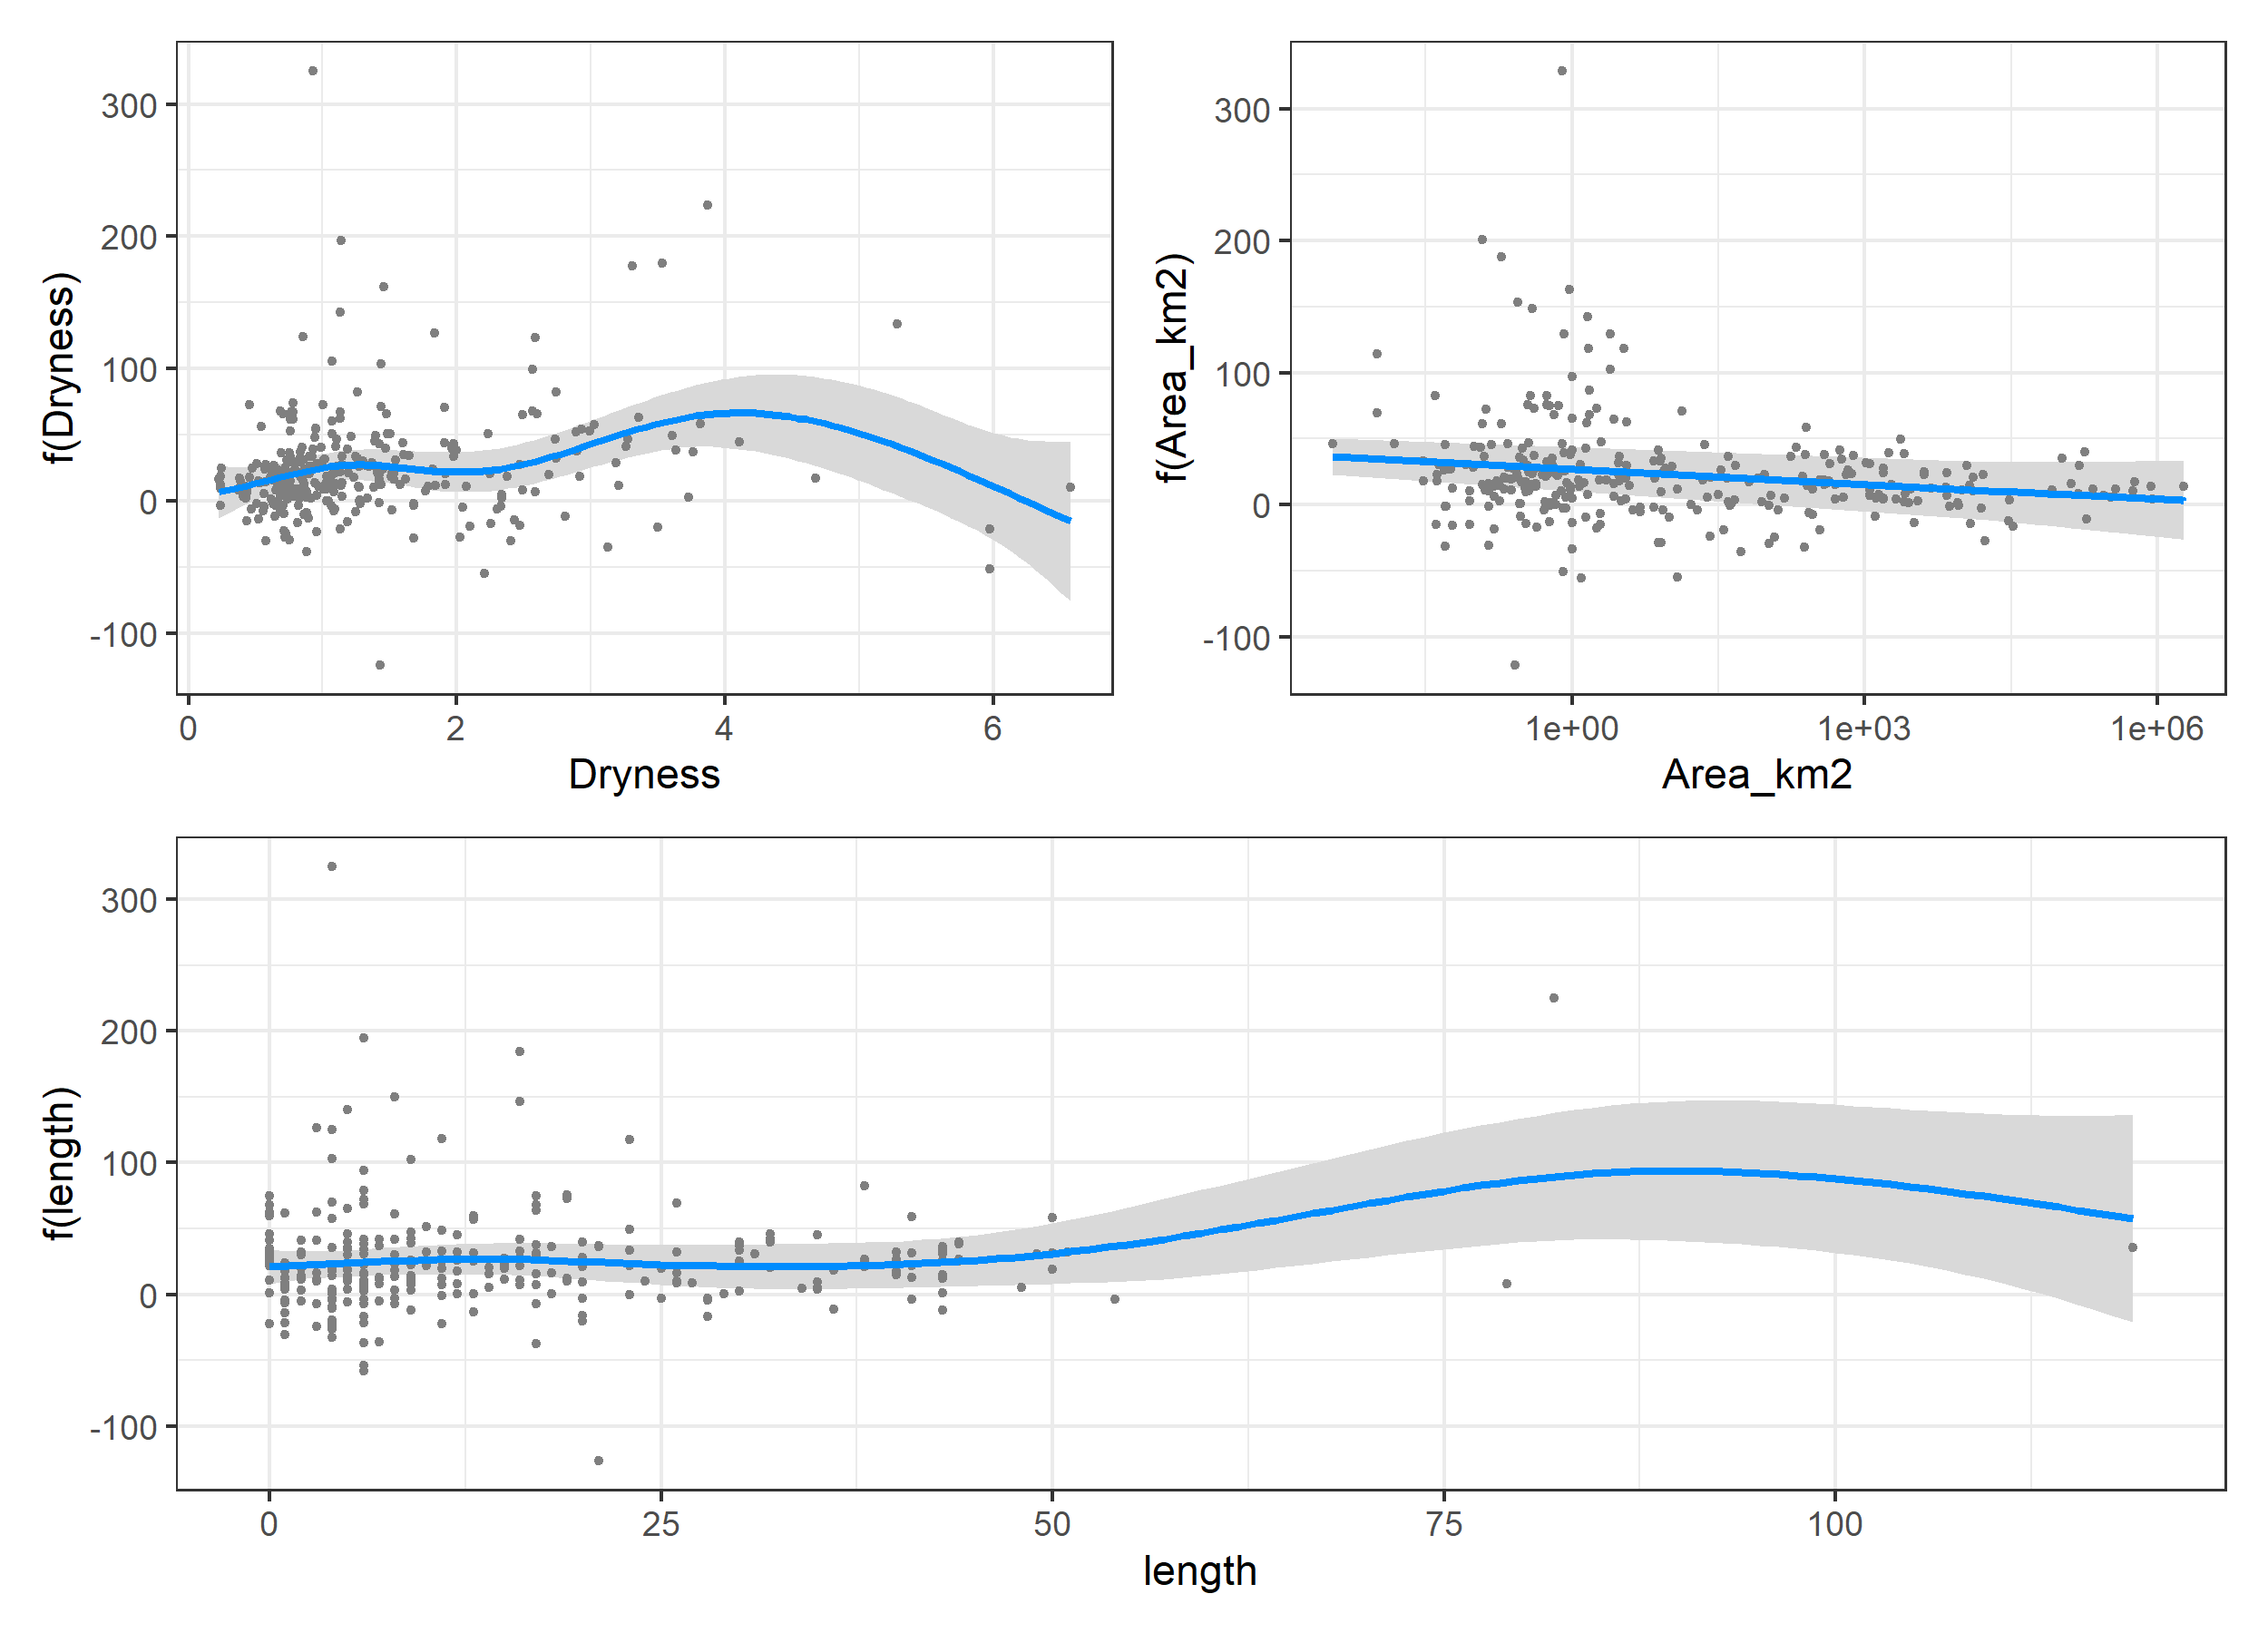
\includegraphics[width=0.9\linewidth]{Forest_model_allsmooths} \caption{Visualisation of the smooth variables in the model, the shaded areas are the 95\% confidence intervals associated with the fit of the smooth, the blue line is the mean smoothed relationship, with data plotted as individual points}\label{fig:smoothsmodelall}
\end{figure}

Figure \ref{fig:smoothsmodelall} highlights that the relationship between \emph{log10(Area km\textsuperscript{2})} and the change in flow is essentially linear. It indicates the negative slope that was also clear from \citet{zhang2017}, indicating that in larger catchments changes in forest cover have less impact on stream flow than for smaller catchments.

Both the \emph{Length} and \emph{Dryness} variables show strong non-linearity, but the relationships do not show a clear trend due to the scatter and the distribution of the data. A further problem appears to be that \emph{Length} and \emph{Dryness} have several points with very high leverage that determine much of the non-linearity in the relationship.

\begin{figure}
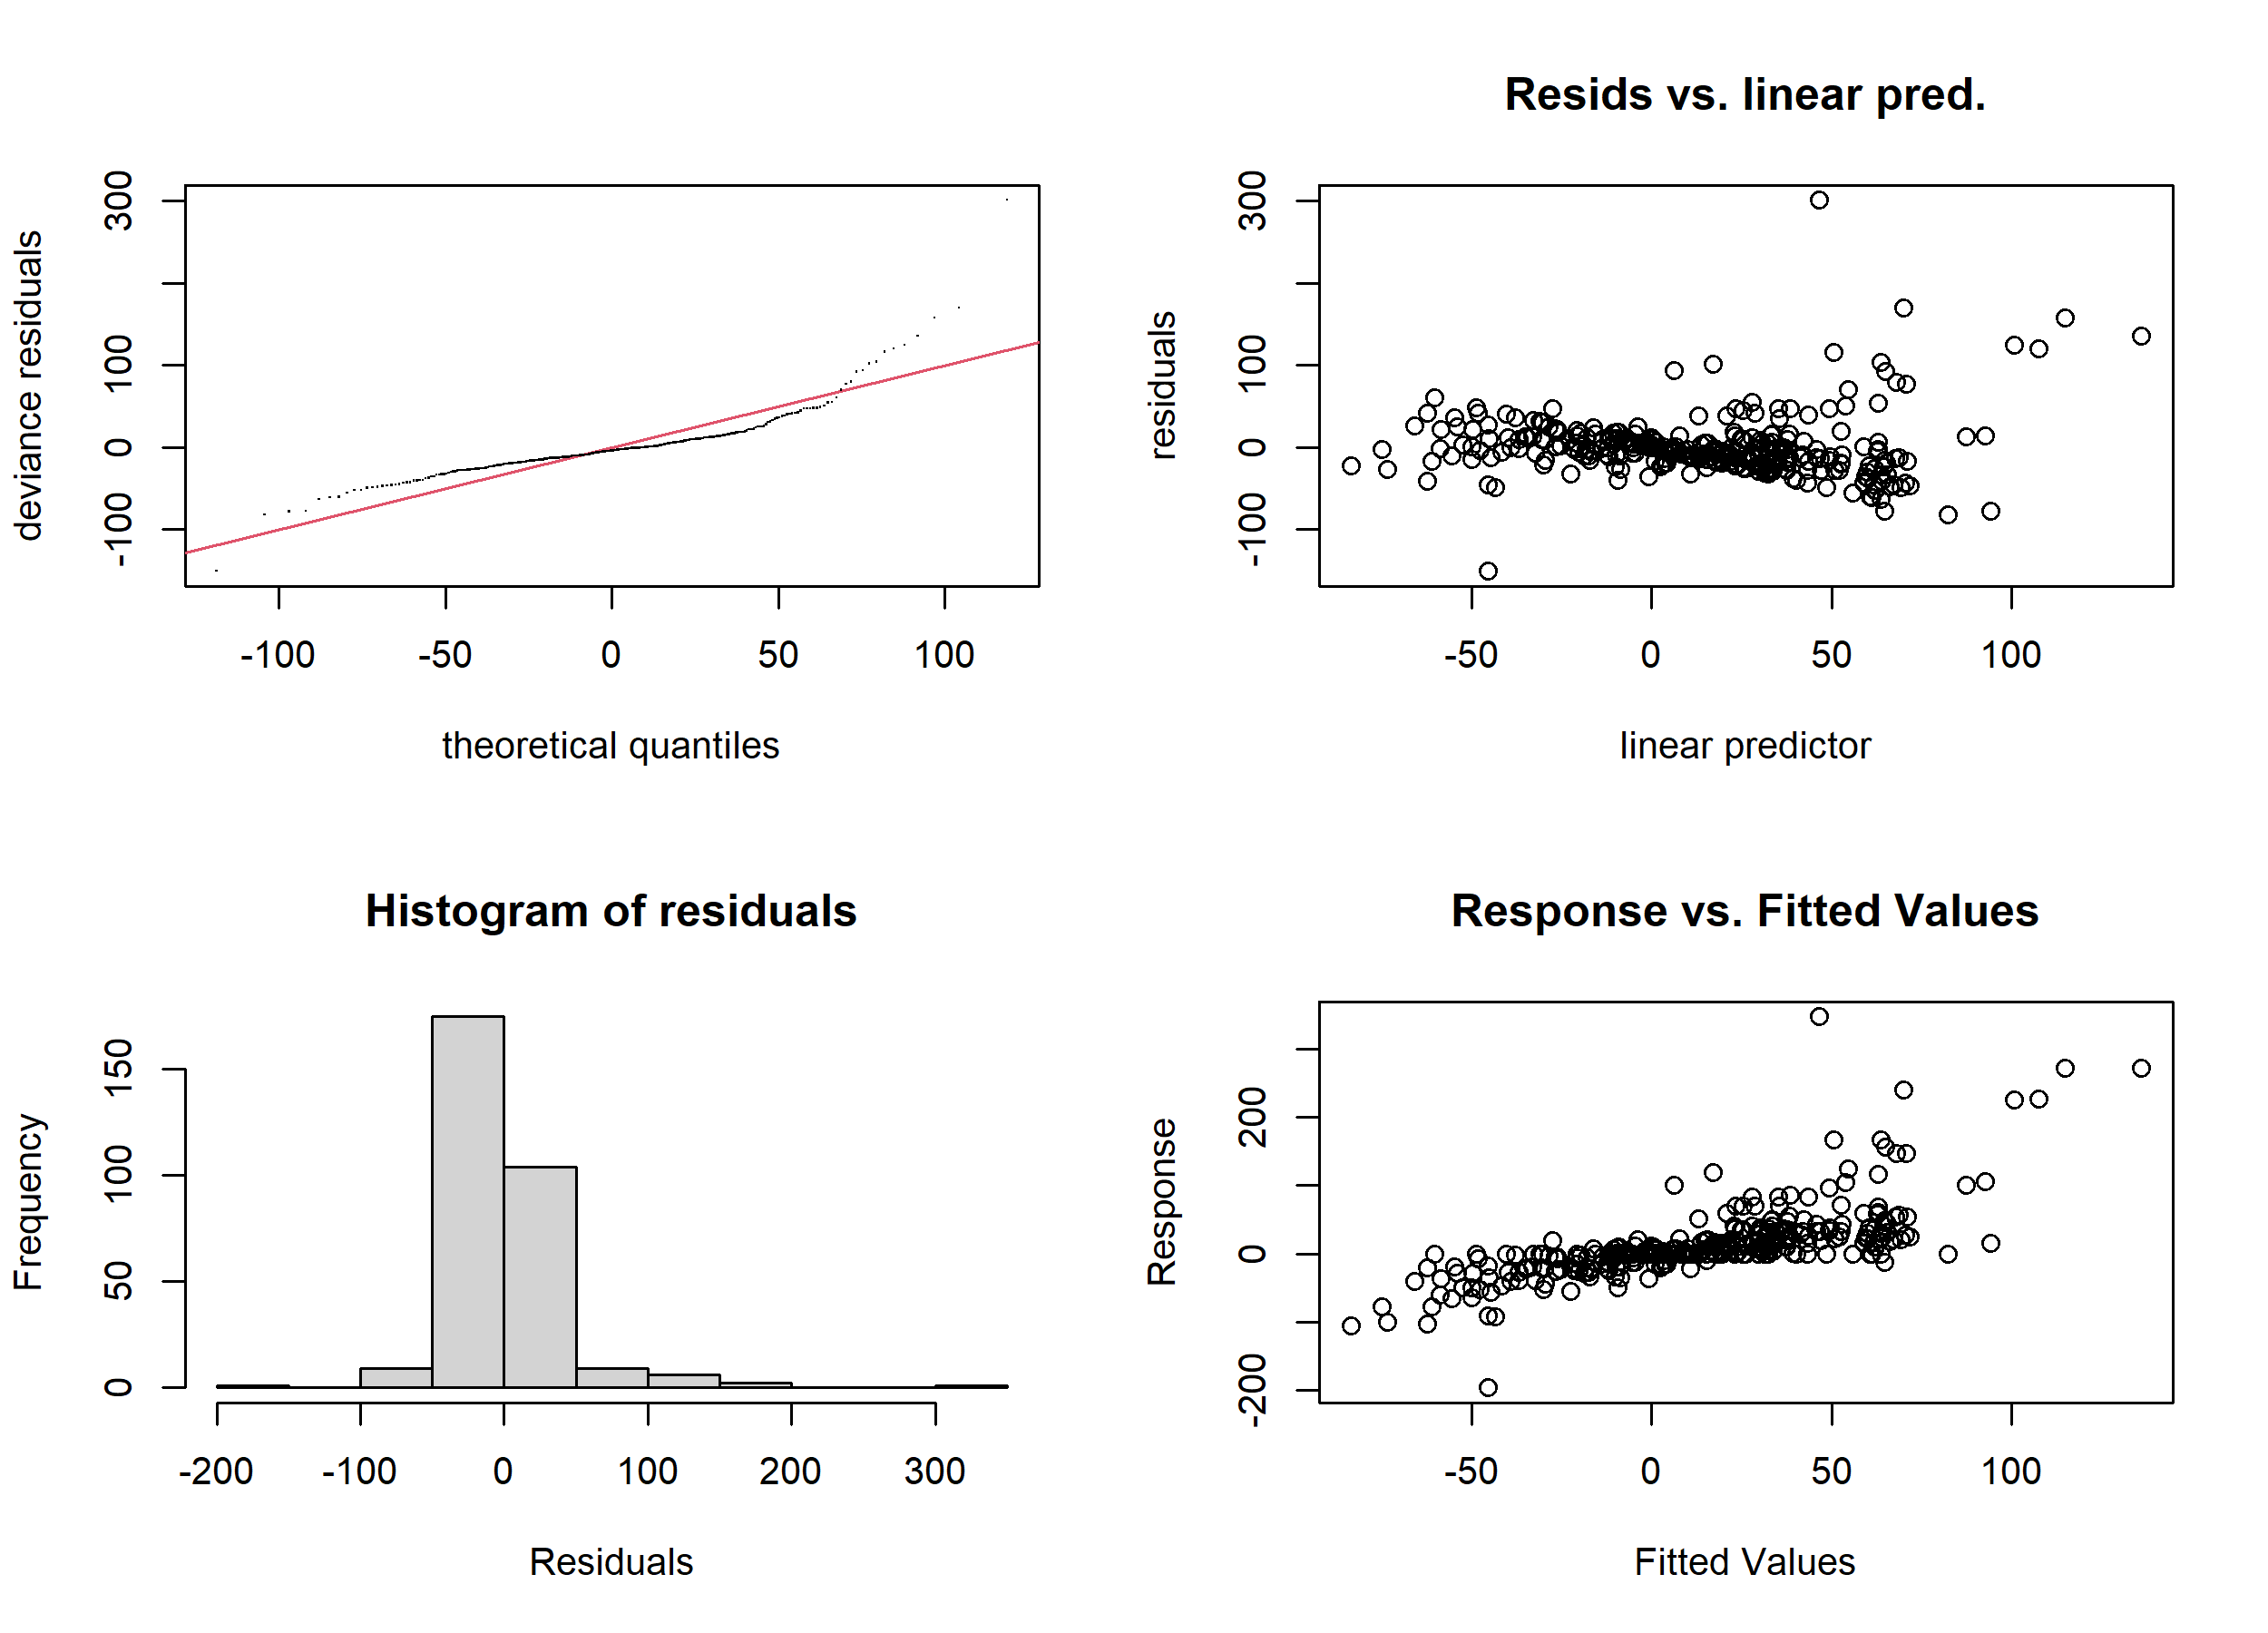
\includegraphics[width=0.9\linewidth]{residual_plot_model_all} \caption{Residual plots for the regression model indicating a slightly fat-tailed residual distribution}\label{fig:gamcheckmodelall}
\end{figure}

As this is not always shown in papers discussing regression relationship, the residual distribution is provided in more detail (Figure \ref{fig:gamcheckmodelall}). Visually, the residuals appear approximately normal, although there is a noticable skew in a limited number of the data in the upper part of the distribution (Figure \ref{fig:gamcheckmodelall}, top left). This is related to a limited number catchments that have very high changes in stream flow in the data set. In other words, the distribution of the residuals is somewhat fat-tailed.

One solution could be to transform the data, however this is not that simple. As the data for the change in flow cover the domain \(\mathbb{R}\), a simple log or Gamma transformation is not a solution. More complex transformations make the results of the regression difficult to interpret, and at some point can be slightly contrived.

Given the majority of the residuals indicate a relatively well behaved distribution, we simply note the behaviour at the extremes and will discuss this later in the paper, and explain how this relates to the characteristics of the data set.

\hypertarget{removal-of-studies-of-great-length-and-for-very-dry-catchments}{%
\subsubsection{Removal of studies of great length and for very dry catchments}\label{removal-of-studies-of-great-length-and-for-very-dry-catchments}}

\begin{longtable}[]{@{}
  >{\centering\arraybackslash}p{(\columnwidth - 6\tabcolsep) * \real{0.1250}}
  >{\centering\arraybackslash}p{(\columnwidth - 6\tabcolsep) * \real{0.1528}}
  >{\centering\arraybackslash}p{(\columnwidth - 6\tabcolsep) * \real{0.1667}}
  >{\centering\arraybackslash}p{(\columnwidth - 6\tabcolsep) * \real{0.3889}}@{}}
\caption{\label{tab:drytable} Catchments for which the dryness index \textgreater{} 5}\tabularnewline
\toprule()
\begin{minipage}[b]{\linewidth}\centering
Number
\end{minipage} & \begin{minipage}[b]{\linewidth}\centering
Latitude
\end{minipage} & \begin{minipage}[b]{\linewidth}\centering
Longitude
\end{minipage} & \begin{minipage}[b]{\linewidth}\centering
Catchment name
\end{minipage} \\
\midrule()
\endfirsthead
\toprule()
\begin{minipage}[b]{\linewidth}\centering
Number
\end{minipage} & \begin{minipage}[b]{\linewidth}\centering
Latitude
\end{minipage} & \begin{minipage}[b]{\linewidth}\centering
Longitude
\end{minipage} & \begin{minipage}[b]{\linewidth}\centering
Catchment name
\end{minipage} \\
\midrule()
\endhead
76 & 34.67 & -111.7 & Beaver Creek, AZ \#3-2 \\
225 & 32.74 & -111.5 & Natural Drainages, Ariz.,
U.S.A, A \\
226 & 32.74 & -111.5 & Natural Drainages, Ariz.,
U.S.A, C \\
356 & -25.75 & 28.23 & Queens river \\
\bottomrule()
\end{longtable}

The flexible nature of the splines means that the Length variable highlights substantial non-linearity in the data, but it is unclear what exactly is captured. The shape of the conditional response (Figure \ref{fig:smoothsmodelall}) does not reflect a similar response as indicated by \citet{filoso2017} and \citet{jackson2005}. One reason could be that the relationship is dominated by the few data points with very long data series, which show highly variable responses (Figure \ref{fig:smoothsmodelall}).

The points related to catchments with very long studies (\textgreater{} 60 years) might be questionable, as changes other than forest cover change could affect stream flow. In addition, a few of the catchments have Dryness values that are very large (\textgreater{} 5) and these values have high leverage in the data, affecting the residual distribution. These catchments are listed in Table \ref{tab:drytable}, and are three catchments in Arizona and 1 catchment in South Africa. It is possible that catchments in these climate zones behave different from the rest of the catchments.

\begin{longtable}[]{@{}
  >{\centering\arraybackslash}p{(\columnwidth - 8\tabcolsep) * \real{0.4231}}
  >{\centering\arraybackslash}p{(\columnwidth - 8\tabcolsep) * \real{0.1410}}
  >{\centering\arraybackslash}p{(\columnwidth - 8\tabcolsep) * \real{0.1667}}
  >{\centering\arraybackslash}p{(\columnwidth - 8\tabcolsep) * \real{0.1282}}
  >{\centering\arraybackslash}p{(\columnwidth - 8\tabcolsep) * \real{0.1410}}@{}}
\caption{\label{tab:m-red-linear} Statistical summary for the linear terms the restricted model}\tabularnewline
\toprule()
\begin{minipage}[b]{\linewidth}\centering
~
\end{minipage} & \begin{minipage}[b]{\linewidth}\centering
Estimate
\end{minipage} & \begin{minipage}[b]{\linewidth}\centering
Std. Error
\end{minipage} & \begin{minipage}[b]{\linewidth}\centering
t value
\end{minipage} & \begin{minipage}[b]{\linewidth}\centering
Pr(\textgreater\textbar t\textbar)
\end{minipage} \\
\midrule()
\endfirsthead
\toprule()
\begin{minipage}[b]{\linewidth}\centering
~
\end{minipage} & \begin{minipage}[b]{\linewidth}\centering
Estimate
\end{minipage} & \begin{minipage}[b]{\linewidth}\centering
Std. Error
\end{minipage} & \begin{minipage}[b]{\linewidth}\centering
t value
\end{minipage} & \begin{minipage}[b]{\linewidth}\centering
Pr(\textgreater\textbar t\textbar)
\end{minipage} \\
\midrule()
\endhead
\textbf{(Intercept)} & -10.69 & 17.85 & -0.6 & 0.55 \\
\textbf{DeltaF\_perc} & -0.61 & 0.08 & -7.69 & 0 \\
\textbf{Forest\_SignIncrease} & 1.12 & 9.72 & 0.12 & 0.91 \\
\textbf{Precip\_data\_typeOB} & -16.23 & 12.46 & -1.3 & 0.19 \\
\textbf{Precip\_data\_typeSG} & 15.96 & 14.86 & 1.07 & 0.28 \\
\textbf{Assessment\_techniqueEA, HM} & 19.97 & 41.02 & 0.49 & 0.63 \\
\textbf{Assessment\_techniqueHM} & 27.07 & 11.39 & 2.38 & 0.02 \\
\textbf{Assessment\_techniquePWE} & 28.54 & 12.11 & 2.36 & 0.02 \\
\textbf{Assessment\_techniquePWE,
HM} & 15.91 & 42.05 & 0.38 & 0.71 \\
\textbf{Assessment\_techniqueQPW} & 43.3 & 19.52 & 2.22 & 0.03 \\
\textbf{Assessment\_techniqueQPW,
EA} & 25.33 & 23.33 & 1.09 & 0.28 \\
\textbf{Assessment\_techniqueSH} & 47.84 & 11.3 & 4.23 & 0 \\
\textbf{Forest\_typeCF} & -7.89 & 7.22 & -1.09 & 0.27 \\
\textbf{Forest\_typeMF} & -6.26 & 7.17 & -0.87 & 0.38 \\
\textbf{Hydrological\_regimeSD} & 0.54 & 8.83 & 0.06 & 0.95 \\
\bottomrule()
\end{longtable}

\begin{longtable}[]{@{}
  >{\centering\arraybackslash}p{(\columnwidth - 8\tabcolsep) * \real{0.3472}}
  >{\centering\arraybackslash}p{(\columnwidth - 8\tabcolsep) * \real{0.0972}}
  >{\centering\arraybackslash}p{(\columnwidth - 8\tabcolsep) * \real{0.1250}}
  >{\centering\arraybackslash}p{(\columnwidth - 8\tabcolsep) * \real{0.0972}}
  >{\centering\arraybackslash}p{(\columnwidth - 8\tabcolsep) * \real{0.1389}}@{}}
\caption{\label{tab:restrictlength} Statistical summary of the smooth terms reducing dataset to studies with the study length shorter than 60 years and Dryness \textless= 5.}\tabularnewline
\toprule()
\begin{minipage}[b]{\linewidth}\centering
~
\end{minipage} & \begin{minipage}[b]{\linewidth}\centering
edf
\end{minipage} & \begin{minipage}[b]{\linewidth}\centering
Ref.df
\end{minipage} & \begin{minipage}[b]{\linewidth}\centering
F
\end{minipage} & \begin{minipage}[b]{\linewidth}\centering
p-value
\end{minipage} \\
\midrule()
\endfirsthead
\toprule()
\begin{minipage}[b]{\linewidth}\centering
~
\end{minipage} & \begin{minipage}[b]{\linewidth}\centering
edf
\end{minipage} & \begin{minipage}[b]{\linewidth}\centering
Ref.df
\end{minipage} & \begin{minipage}[b]{\linewidth}\centering
F
\end{minipage} & \begin{minipage}[b]{\linewidth}\centering
p-value
\end{minipage} \\
\midrule()
\endhead
\textbf{s(Dryness)} & 3.82 & 9 & 2.15 & 0 \\
\textbf{s(log10(Area\_km2))} & 0.89 & 4 & 1.66 & 0.01 \\
\textbf{s(Length)} & 0 & 9 & 0 & 0.97 \\
\bottomrule()
\end{longtable}

\begin{figure}
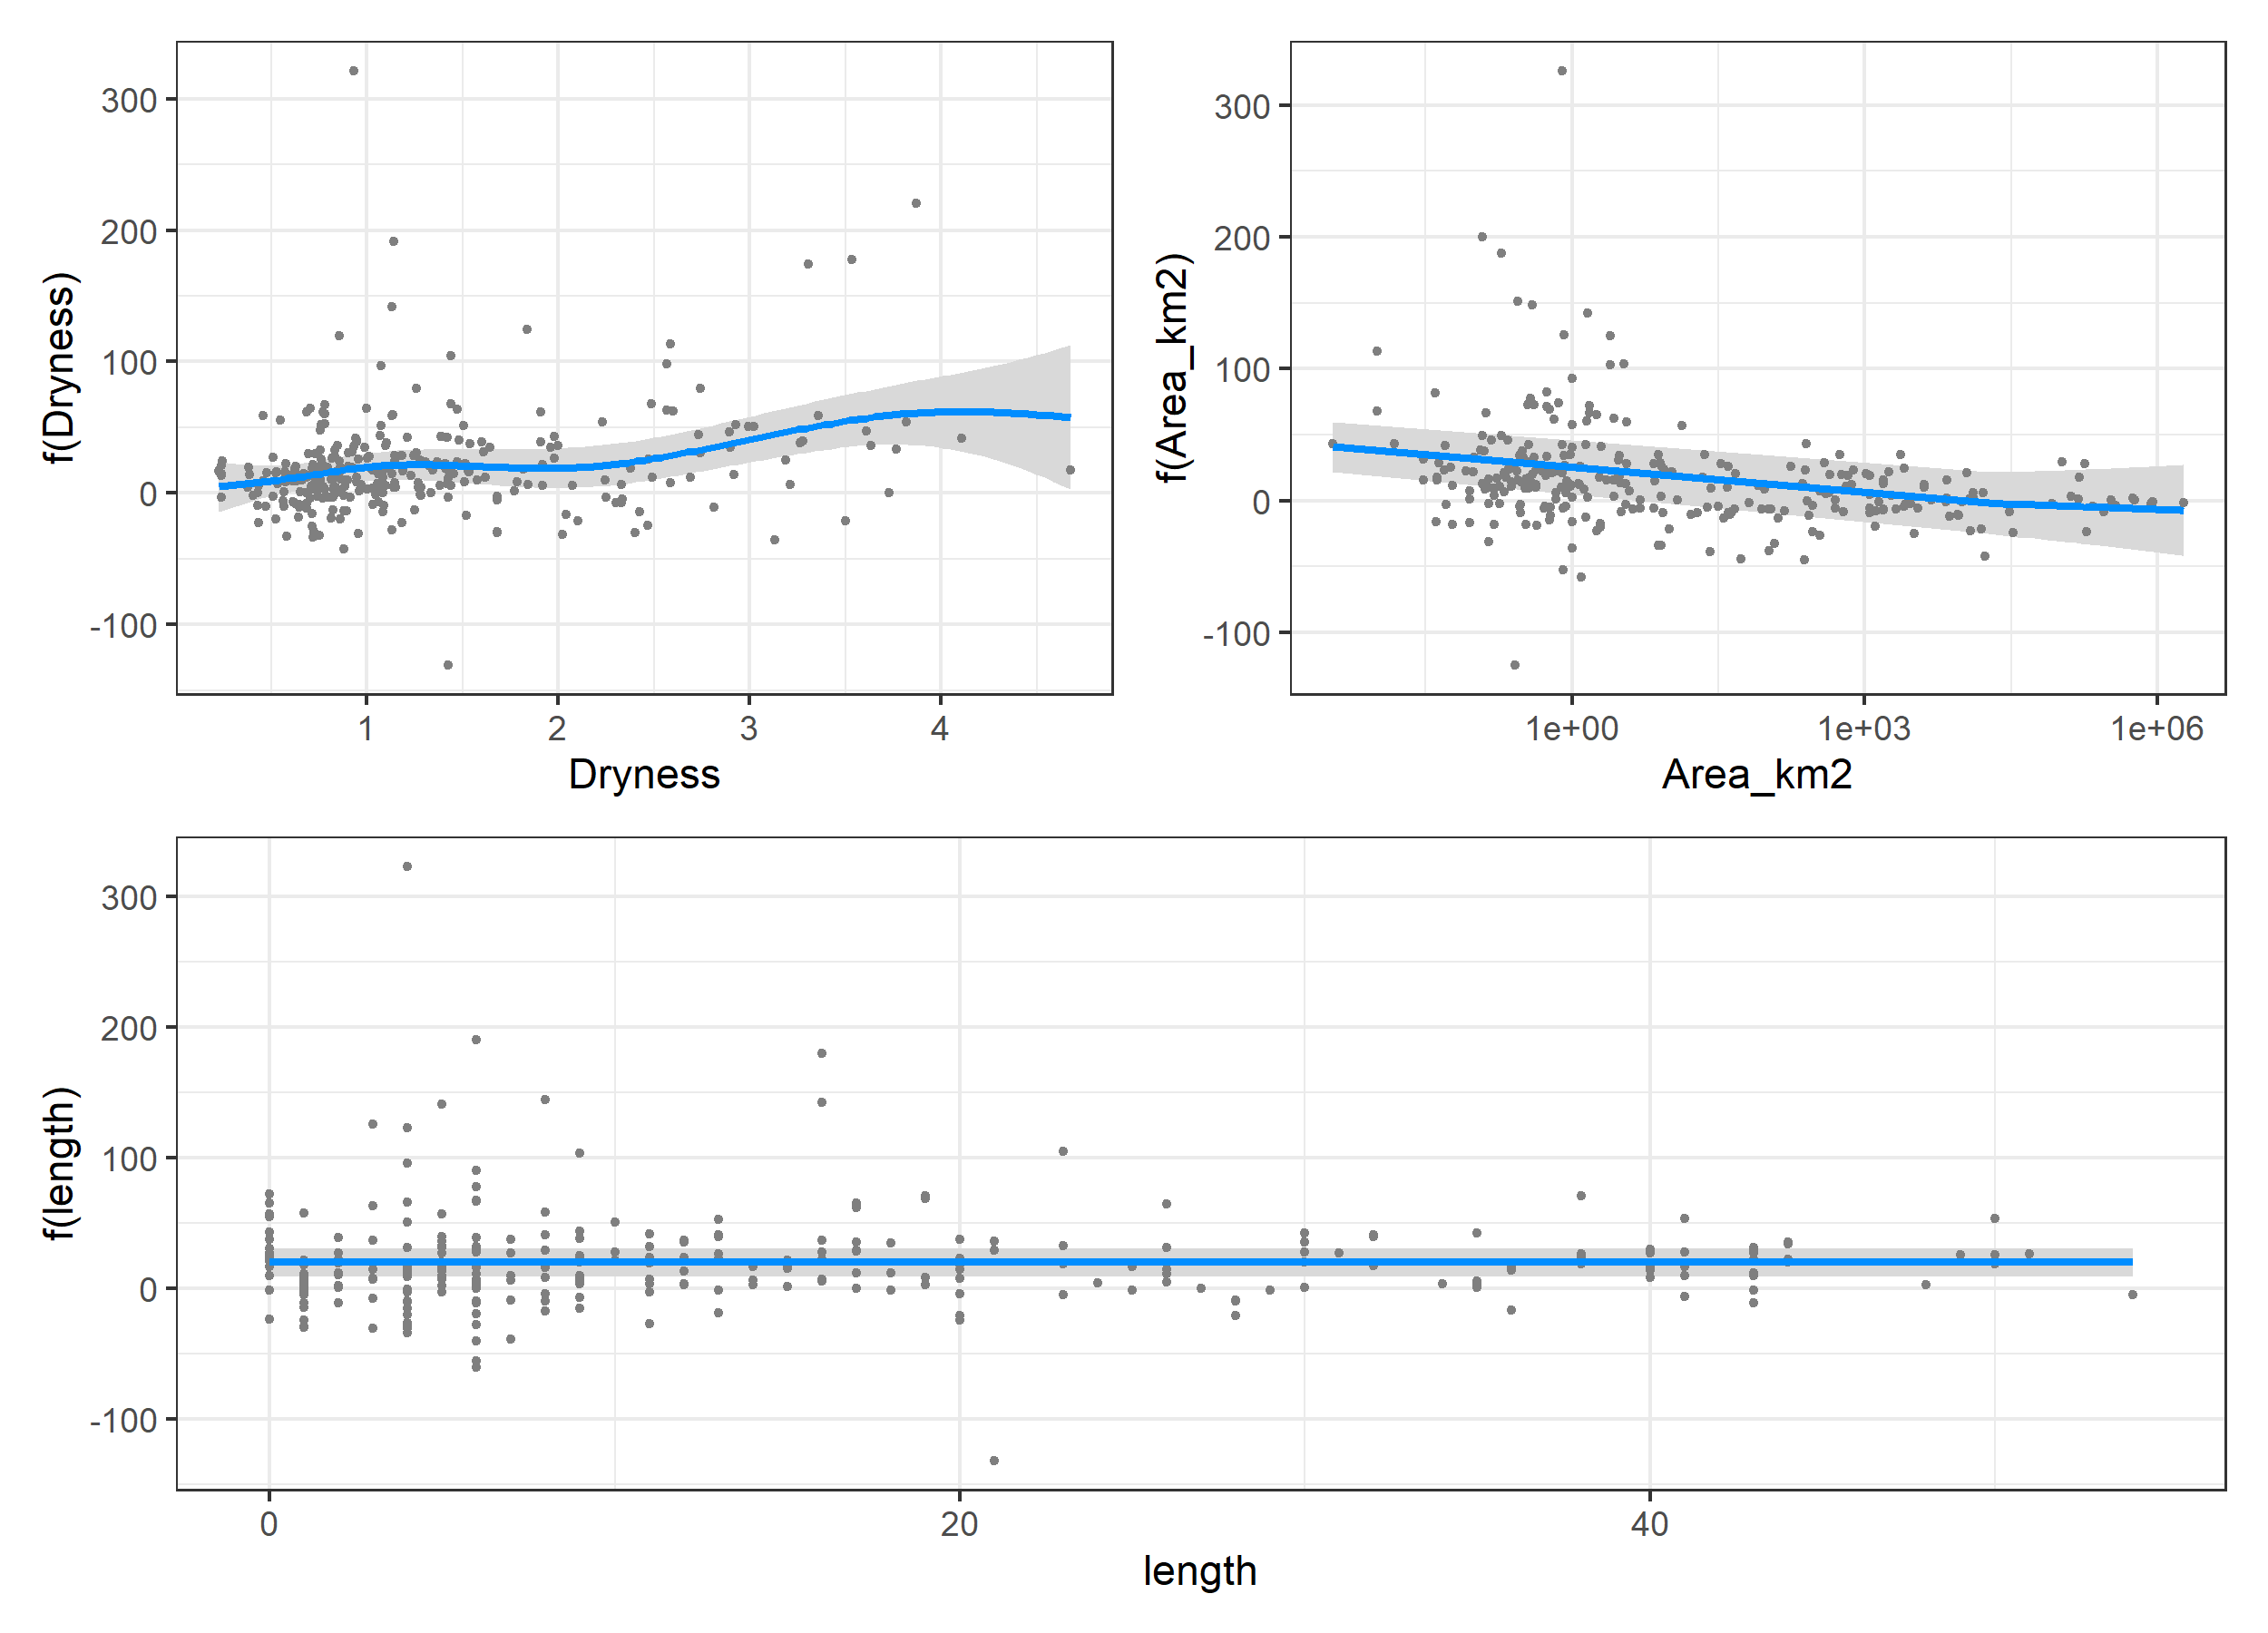
\includegraphics[width=0.9\linewidth]{model_redLength_smooths} \caption{Visualisation of the smooth variables in the model with reduced data for dryness and length}\label{fig:smoothsmodelredLength}
\end{figure}

Therefore it is worth investigating what effect removing these few data points has on the overall model and the significance of the variables. Data that have \emph{Dryness} \textless= 5 and \emph{Length} \textless= 60 years were removed from the data set and the model based on a reduction of the data set from 334 to 315 catchments is run again.

This model, which excludes data with long studies and very dry catchments explains only slightly less of the variation with an adjusted \emph{r\textsuperscript{2}} of 0.45 and a deviance explained of 0.48.

Investigating the non-linear responses suggest that \emph{Dryness} has a clear non-linear response, which is significant, where changes in forest cover in drier catchments having a greater impact on stream flow (Figure \ref{fig:smoothsmodelredLength} and Table \ref{tab:restrictlength}). Catchment area (\emph{log10(Area (km\textsuperscript{2}))}) still has an impact on flow with p = 0.01, and the relationship looks almost linear. More importantly, the variable \emph{Length} is no longer significant, after removal of the two studies with very long lengths.

\begin{longtable}[]{@{}
  >{\centering\arraybackslash}p{(\columnwidth - 2\tabcolsep) * \real{0.3194}}
  >{\centering\arraybackslash}p{(\columnwidth - 2\tabcolsep) * \real{0.0833}}@{}}
\caption{\label{tab:tableassess} Distribution of assessment techniques in the data set}\tabularnewline
\toprule()
\begin{minipage}[b]{\linewidth}\centering
Assessment\_technique
\end{minipage} & \begin{minipage}[b]{\linewidth}\centering
n
\end{minipage} \\
\midrule()
\endfirsthead
\toprule()
\begin{minipage}[b]{\linewidth}\centering
Assessment\_technique
\end{minipage} & \begin{minipage}[b]{\linewidth}\centering
n
\end{minipage} \\
\midrule()
\endhead
PWE & 187 \\
HM & 57 \\
SH & 45 \\
EA & 32 \\
QPW & 7 \\
QPW, EA & 4 \\
EA, HM & 1 \\
PWE, HM & 1 \\
\bottomrule()
\end{longtable}

One concern with the results presented so far is that there are a few assessment techniques in the data set with a very low number of observations and could influence the results of the analysis. This includes the category of Quasi paired watersheds and combinations of elasticity analysis and hydrological modelling (EA,HM) and paired watersheds and hydrological modelling (PWE,HM) (Table \ref{tab:tableassess}).

Therefore, the model was rerun excluding the combined assessment techniques (EA, HM), (PWE, HM) and (QPW, EA) and the assessment technique QPW, which were all non-significant (Table \ref{tab:tableassess}). This resulted in a data set of 328 catchment studies.

The model based on assessment techniques that have more than 10 observations in the data set does not change much in the results (results not shown). It strengthens the significance of the different assessment techniques, but generally results in the same interpretation. Overall this suggests that although those observations have some impact on the overall relationships, they do not strongly bias the outcomes.

The overall model results clearly highlight that some of the assessment techniques (in particular paired watershed studies (PWE) and combined use of statistical methods and hydrographs (SH)), have a strong impact on the predicted change in flow. Particularly, relative to EA (elasticity approaches) all other assessment techniques have higher predicted changes in flow. In other words, there is a distinct difference in the way the change in flow is assessed, and the EA method (for example in \citet{zhou2015}) appears to suggest a much smaller effect on the change in flow.

\hypertarget{discussion}{%
\section{Discussion}\label{discussion}}

The generalized additive models appear to reach the same conclusions as the single variable regression in earlier papers \citep{zhang2017, filoso2017}. It appears that:

\begin{enumerate}
\def\labelenumi{\arabic{enumi}.}
\tightlist
\item
  Larger catchments show lower impact of forest cover change on stream flow;
\item
  Drier catchments show a greater impact of forest cover change on stream flow; and
\item
  There is a general linear relationship between the change in forest cover and the change in stream flow.
\end{enumerate}

This might suggest that the simpler models have reached the correct conclusion. However, this is somewhat premature. given that the other major point coming out of the results is:

\begin{enumerate}
\def\labelenumi{\arabic{enumi}.}
\setcounter{enumi}{3}
\tightlist
\item
  There is a clear relationship between size of catchments, area cleared and type of experiments, with particular Paired Watershed Experiments containing the smallest catchments, the largest percent forest cover change and the largest variability in the flow response.
\end{enumerate}

\begin{figure}
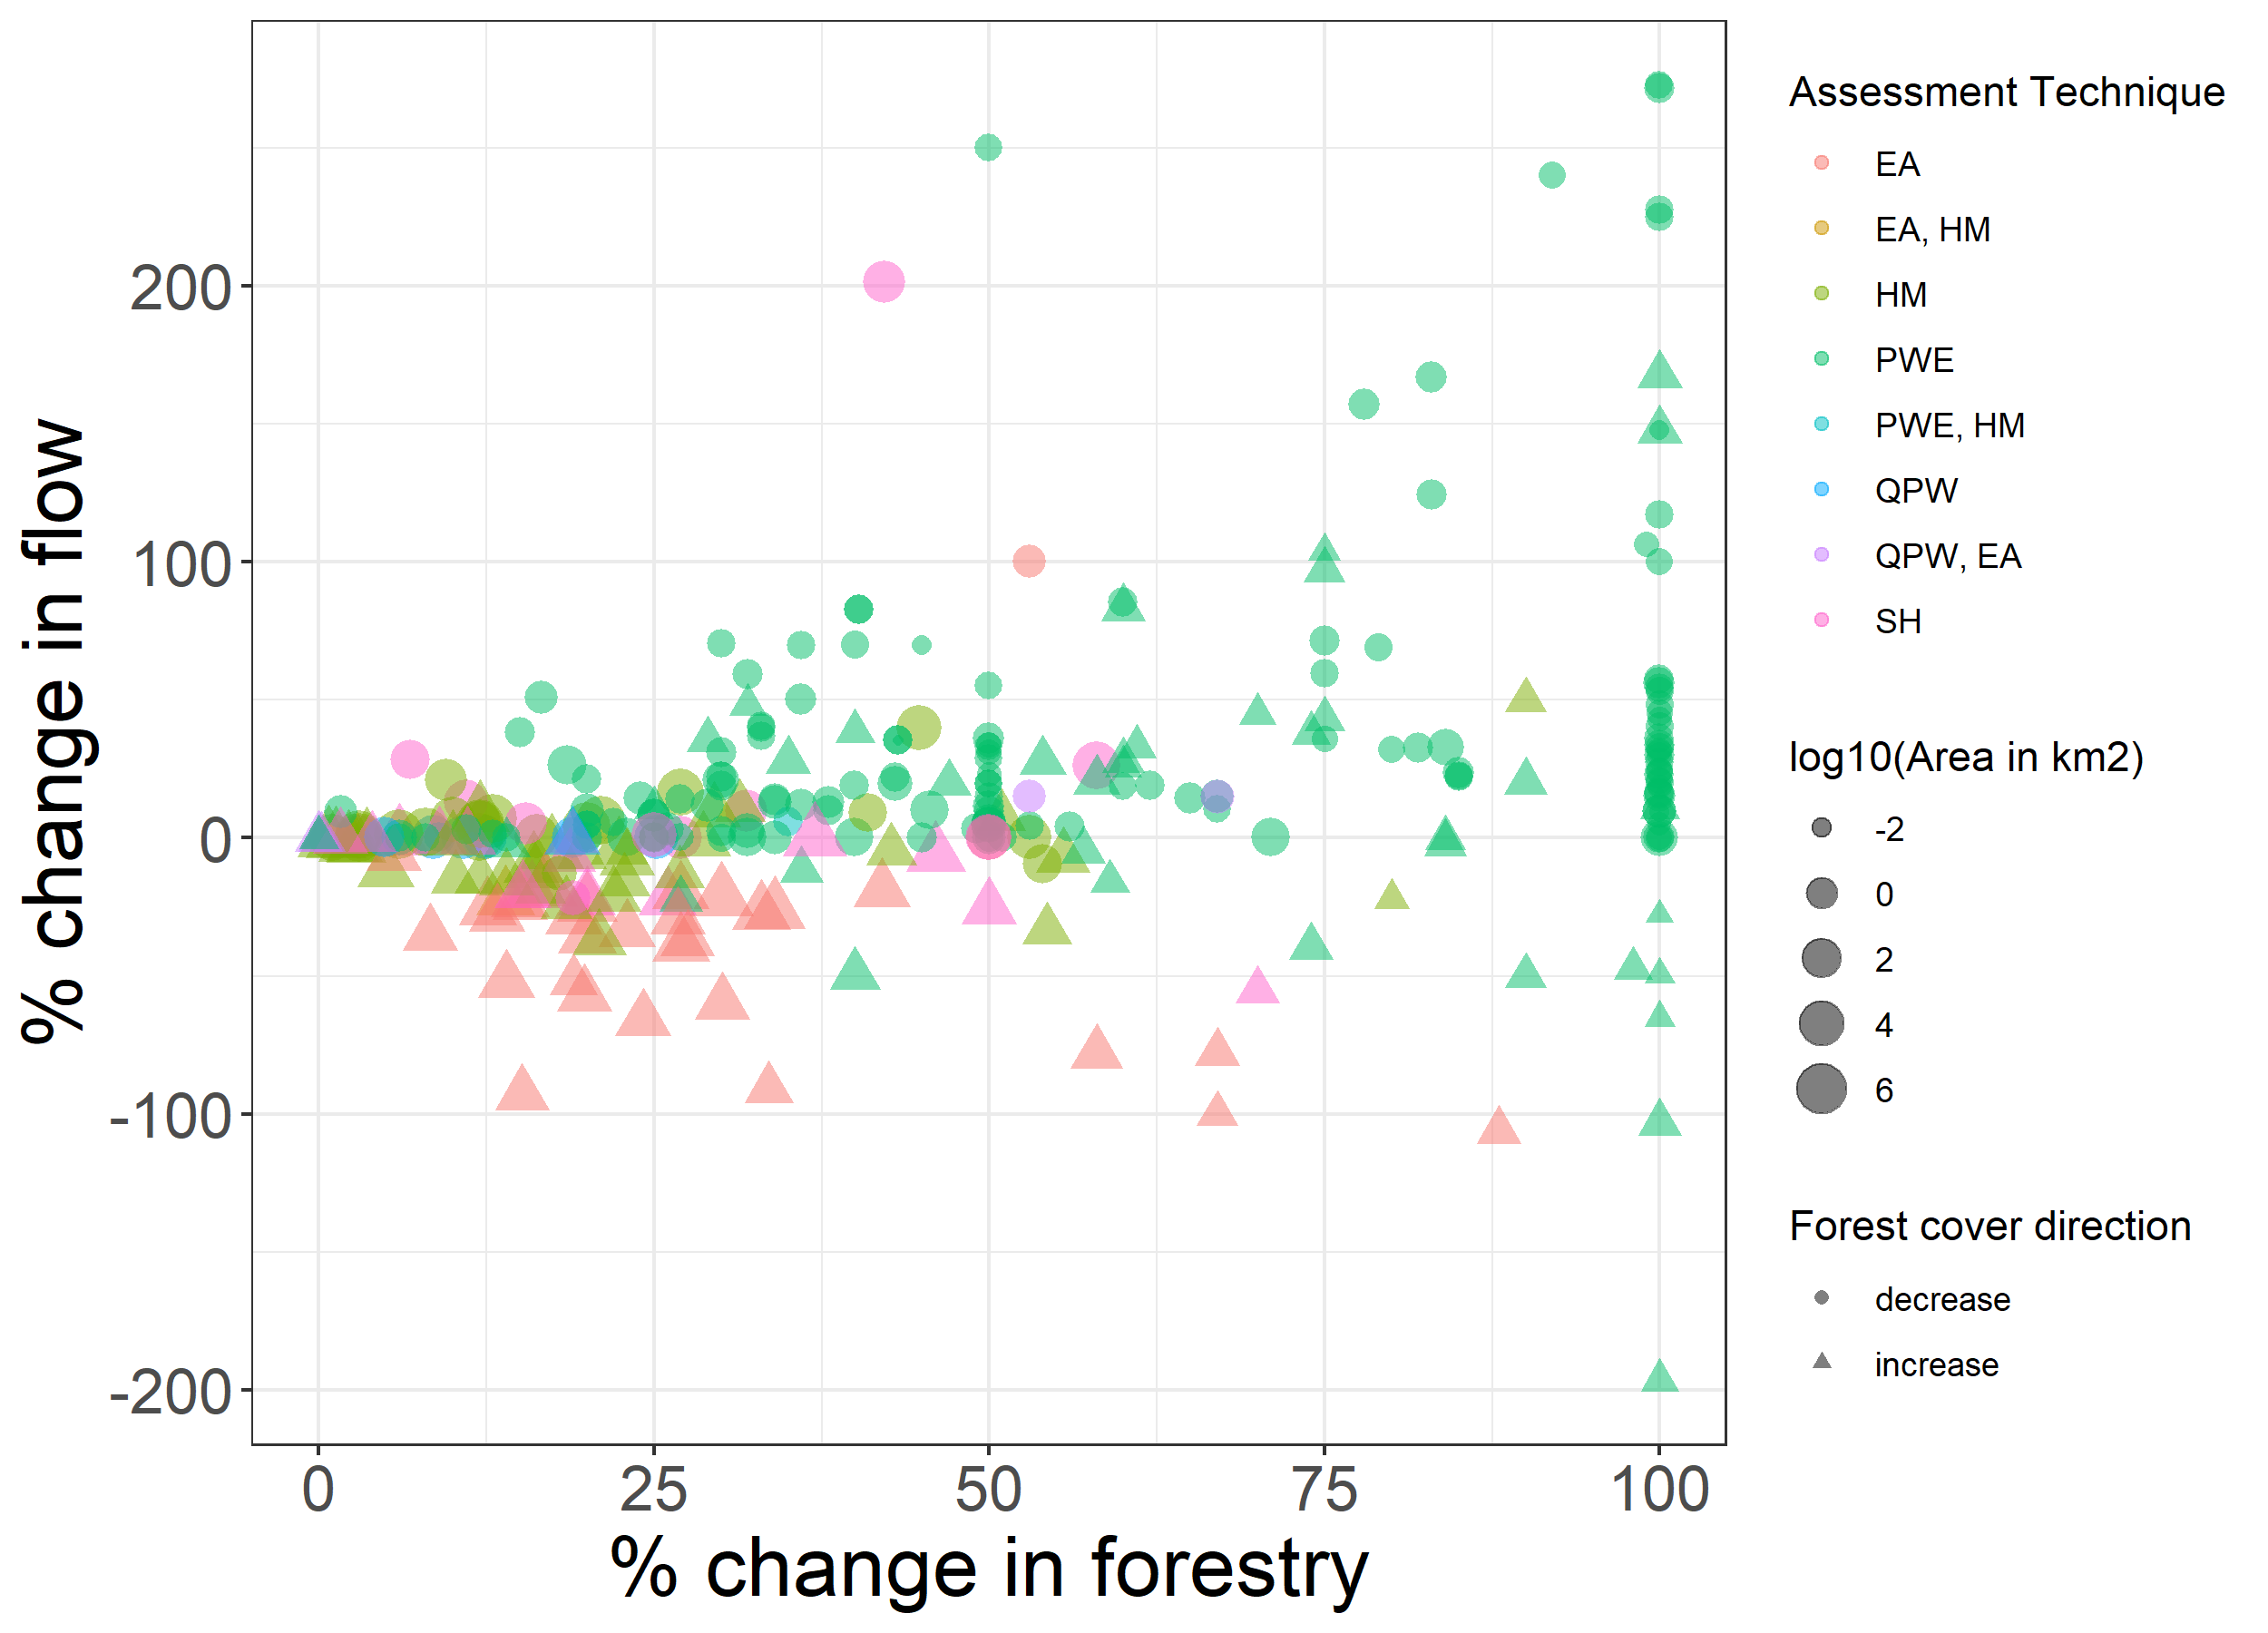
\includegraphics[width=0.9\linewidth]{flow_forest_byArea} \caption{Overview of the data highlighting the dominance of small catchment studies which are fully forested or cleared and the scatter in the data}\label{fig:overview}
\end{figure}

Figure \ref{fig:overview} provides a clear overview of the whole data set, and in this figure the size of the catchments and the different assessment methods are highlighted. This figure clearly indicates that the data relating to high changes in forest cover are all small catchments and relate mostly to paired watershed experiments. In contrast, data related to large catchments are related to smaller changes in forest cover and different methods, such as hydrological modelling and elasticity analysis. This confirms the model results (Table \ref{tab:m-red-linear}) and the earlier correlation analysis (Figure \ref{fig:corgraphs}).

It is possible that one of the reasons why \citet{zhang2017} separated their analysis in large (\textgreater{} 1000 km\textsuperscript{2}) and small (\textless{} 1000 km\textsuperscript{2}) catchments, is that they realized this difference in assessment methods and wanted to account for this. However, this is not explicitly identified, and there is no real physical explanation of the 1000 km\textsuperscript{2} threshold.

The other interesting point in Figure \ref{fig:overview} is that the variation in the data increases as the catchment size decreases and the change in forest cover increases. This also means that the overall variation in the data for paired watershed experiments (PWE) is much greater than for any of the other methods.

\hypertarget{is-there-a-problem-with-extending-local-experimental-data-to-larger-scales}{%
\subsection{Is there a problem with extending local experimental data to larger scales?}\label{is-there-a-problem-with-extending-local-experimental-data-to-larger-scales}}

The overarching reason for combining past studies at a global scale is to infer relationships that can be used to make more general statements or develop more global scale modelling of impacts \citep[i.e.][]{zhou2015, jackson2005, hoekvandijke2022}. Therefore, the results from the analysis could be seen as a confirmation of the earlier research \citep{zhang2017, filoso2017, zhou2015, jackson2005}. However, the explaining power of the developed model is quite low and a lot of variation in the data is unexplained. As is highlighted in the introduction there are four major issues with this type of analysis, and the results from this paper also highlight these issues. Here, these issues are further explained.

\hypertarget{issue-1-latent-variables-are-not-included-in-the-typical-single-covariate-analysis}{%
\subsubsection{Issue 1: Latent variables are not included in the typical single covariate analysis}\label{issue-1-latent-variables-are-not-included-in-the-typical-single-covariate-analysis}}

The results show that it is simply impossible to analyze a single covariate relationship, as there are several latent variables in the data. An example of this is the general relationship of the change in flow as a function of the change in forest cover. Clearly the relationship is highly impacted by the fact that all the small catchments have large changes in forest cover and are all associated with paired watershed experiments. Without taking these factors into account, a definite answer about the impact of forest cover on the change in flow cannot be given. Furthermore, the large variability in the change in flow data for these small catchments (Figure \ref{fig:overview}) indicates that there is a further (unknown) variable that explains the variation in the data.

If the remaining variation in the residuals is small relative to the trend, then there is little need to identify further latent variables, but if the variation is large, then it is unclear if it is the latent variable that determines the trend, or the actual relationship in the data.

Similarly, the data for the larger catchments containing smaller changes in forest cover are dominated by hydrological modelling studies, resulting in a further complication. If the reponse of the stream flow in the modelling studies is the result of the conceptualized relationship between stream flow and forest cover (possibly from a subset of the paired catchment studies), then it is impossible to say if the change in stream flow is real, or simply a result of a pre-conceived model relationship. Is the smaller variation in the data for smaller changed in forest cover (Figure \ref{fig:overview}) a result of similar conceptualized model relationships, or actual variation between catchments and climate types? Currently this question cannot be answered.

This becomes problematic when extrapolated to larger scales. A clear example of this is the paper by \citet{hoekvandijke2022} where the conceptualized relationship between forest cover and stream flow pre-determines the outcomes of the global modelling.

The only way to analyze changes in stream flow as a function of forest cover in larger catchments is to actually derive this from observed data of long term stream flow and forest cover (as was done in \citet{levy2018}).

One of these latent variables could be the total area of forest in a catchment, as was analysed in \citet{levy2018}. In this case, the total \% area of forest was not included in the data. As a test, the total \% area of forest for the larger catchments (\textgreater{} 1000 km\textsuperscript{2} in \citet{zhang2017}) were added to the data set and the model for just the large catchments was tested. This showed that the \% area of forest was not significant to explain the change in flow for the larger catchments (retaining all other variables in the model, results not shown). While this might be an area of further research on the full data set, it is complicated for two reasons:

\begin{enumerate}
\def\labelenumi{\arabic{enumi}.}
\tightlist
\item
  The area of forest is not always indicated in the original papers, or a range of values is given, complicating the data collection.
\item
  Many of the small catchments have 100\% area covered in forest, introducing a strong skew in the data and complicating if total area of forest has an impact on the change in flow.
\end{enumerate}

We are not arguing that there is no relationship between stream flow and forest cover, and there might indeed be a global relationship that can be discovered. But, this relationship can only be discovered if we are able to address some of the major other factors that explain the variability, and work with actual data and not model outputs.

\hypertarget{issue-2-interpretation-errors-due-to-complex-descriptions-of-the-experiments-in-the-original-papers}{%
\subsubsection{Issue 2: Interpretation errors due to complex descriptions of the experiments in the original papers}\label{issue-2-interpretation-errors-due-to-complex-descriptions-of-the-experiments-in-the-original-papers}}

The second major issue that became clear from reviewing many of the original papers is that some of the variability might be an interpretation problem. In many cases the original description in the paper is interpreted to extract the \% change in stream flow from the \% change in forest cover. This seems like a simple activity, but this is not always the case.

Two examples can be highlighted:

\begin{itemize}
\tightlist
\item
  The papers from \citet{almeida2016} and \citet{ferreto2020} partly discuss the same experiment and the same catchment. In \citet{almeida2016}, the methods discuss how two experimental catchments of approximately 80ha in size which were harvested. One catchment was 100\% harvested and the other 30\% harvested. Throughout the paper the catchments are indicated as 100\% harvested and 30\% harvested. However, only after reading \citet{ferreto2020}, did we discover that in fact the 100\% and 30\% refer to the ``eucalyptus plantation area'', which was about 60\% of the total area. This is in fact mentioned in Table 1 in \citet{almeida2016}, but does not appear in the text. The question then becomes how to interpret this in the data base for this paper. Clearly it was a 100\% and 30\% change in forest cover, but only for the 60\% plantation cover, not for any of the other areas in the catchment, which included native vegetation and riparian vegetation. There are several other examples like this in the different papers \citep[for example][]{blackie1979kimakia, blackie1979kericho}.
\item
  Another example is the paper by \citet{waterloo2007}. This modelling study in Fiji of the clearing of a catchment reports the changes in stream flow over parts of the year. For a period of 324 days the stream flow increased from 252 mm to 580 mm (a 230\% increase if calculated as \(580/252*100\)) and for a second period of 309 days the stream flow increased from 90 mm to 194 mm (a 215 \% increase). However, how we convert this to a change in annual flow (which most of the other data relate to) is difficult. The original data base listed a 50 \% change in flow, but it is difficult to identify how this is calculated. We suspect that results from \(252/580*100 \approx 50\) and \(90/194 \approx 50\).
\item
  A final example is around the choice of control or treatment. In the data base the assumption is that the change in flow is relative to the original situation. This can be either a ``before and after'' analysis, which can be problematic by itself due to climate variation, or a comparison of a treatment with a control. But even in this case comparing across catchments can be tricky. For example, at one extreme, some controls in the database are a bamboo catchment and a tea plantation \citep{blackie1979kimakia, blackie1979kericho}. A clearer example is the Brigalow catchment study in Queensland, Australia \citep{thornton2007brigalow}, catchment \#336 in the data set. This is a paired watershed experiment of conversion of native Brigalow (an Acacia species) into cropland and pasture. We chose to use the cropped catchment (C2 \citet{thornton2007brigalow}) as the deforestation treatment resulting in a change of flow of 140\%, based on Table 4 in \citet{thornton2007brigalow}. However, had we used the pasture catchment as the treatment then the change in flow would have been up to 165\%.
\end{itemize}

Clearly, interpreting older papers can be difficult and this can result in variation in the data that is being analyzed. Similar to the last issue, if these errors only introduce small variation in the data, then it will not limit the interpolation to larger scales. At this point, it is not clear if this is indeed the case. The large variation in the experimental watershed data suggests that this might be a more serious problem.

\hypertarget{issue-3-aggregation-of-data-that-originates-from-different-experiments-with-different-objectives-across-a-wide-time-period}{%
\subsubsection{Issue 3: Aggregation of data that originates from different experiments with different objectives across a wide time period}\label{issue-3-aggregation-of-data-that-originates-from-different-experiments-with-different-objectives-across-a-wide-time-period}}

For many of the small catchment studies listed in the database, the assumption is that the original experimental design can be interpreted in terms of a binary ``forestation'' or ``deforestation''. However, the real situation is often much more complex and fuzzy.

Many of the paired watershed experiments included a harvesting and replanting or regrowth after harvesting or fire experiment \citep[e.g.][]{cornish1993, cornish2001, webb2013}. As a result, it becomes difficult to assess how we interpret the change in flow as a result of a change in cover. In many cases we would expect the flow to change over time as a function of the recovery \citep{jones2017} and therefore the time series of the flow needs to be assessed over a longer time.

Many of the papers in the database report early results (for example 1 or 3 years after harvesting), but some also report longer time periods. As earlier work \citep{cornish2001, jones2017} has highlighted, we can always expect a larger effect directly after harvesting, but this effect diminishes over time (even if it does not always return to the original state). Comparing studies reporting results directly after treatment to longer term studies therefore becomes problematic.

In our work, the variable \emph{Length} was used in the model to test for some of these effects, but this was insignificant in the model (Table \ref{tab:restrictlength}). Given the other variation in the data, this does not necessarily mean that there is no effect.

This is further complicated by the variation in different types of clearing and the different types of vegetation. In the original \citet{zhang2017} a variable to describe the \emph{forest type} was included (Table \ref{tab:table1}), but in the model this is not significant (Table \ref{tab:m-all-linear}). This is probably because the broad classification used does not capture the actual variation in runoff response. In addition, as Figure \ref{fig:corgraphs} shows, there is a correlation between coniferous forests and snow dominated hydrological regimes, further complicating the analysis.

An additional complication related to combining studies related to wild fires or bush fires and logging studies is the differences in vegetation recovery. For example, \citet{heath2014} found that catchments with resprouting species around Sydney, Australia, indicated little change in the stream flow in comparison to species regrowing from seed further south on the continent \citep{zhou2015bushfire}.

As a result, it can be difficult to exactly pinpoint the change in flow as a result of the change in cover, as well as being difficult to assess what the exact change in cover actually was. In addition, using only the overall change in stream flow can discard a lot of information from observations in individual years. Many papers give stream flow values for multiple years, often showing significant variation. Summarizing this into one average value discards all the information on the variance.

As indicated before, if the overall variation in the data due to this issues is small, then this would not be an issue for upscaling the results, but the large variation for the smaller catchments suggest that effects could be considerable. As \citet{jones2017} indicate, this really needs time series analysis of the different experiments. However, some of the time series data might not be recoverable from the older experiments, which will limit the opportunities for analysis. We will discuss this further below.

\hypertarget{issue-4-transcription-errors-in-the-data}{%
\subsubsection{Issue 4: Transcription errors in the data}\label{issue-4-transcription-errors-in-the-data}}

This issue seems to mainly occur if data is collected from other review papers. This might be because some of the original papers are difficult to locate and therefore values from reporting papers are used. In supplementary data part 1, several changes to the original data sets have been documented, and as can be seen several of these are transcription errors.

This does influence the results in \citet{zhang2017}, comparing the results in Supplementary material 2 with the original paper. The main example is that in this study the largest catchment (watershed \#1 in \citet{zhang2017}) had to be removed, as this study actually involved paired watershed experiments on very small plots, for which the characteristics were not recoverable.

Clearly, this is a problem for all reviews that attempt to bring together large numbers of results from published papers, and where actual results are copied rather than using some sort of automated text analysis.

In the end, careful review of the data and the original papers can circumvent most of this issue. And, making the data available (as \citet{zhang2017}, \citet{zhou2015}, \citet{filoso2017} and this paper have done) provides an opportunity for review by other researchers, and over time most of the transcription errors can be resolved.

\begin{figure}
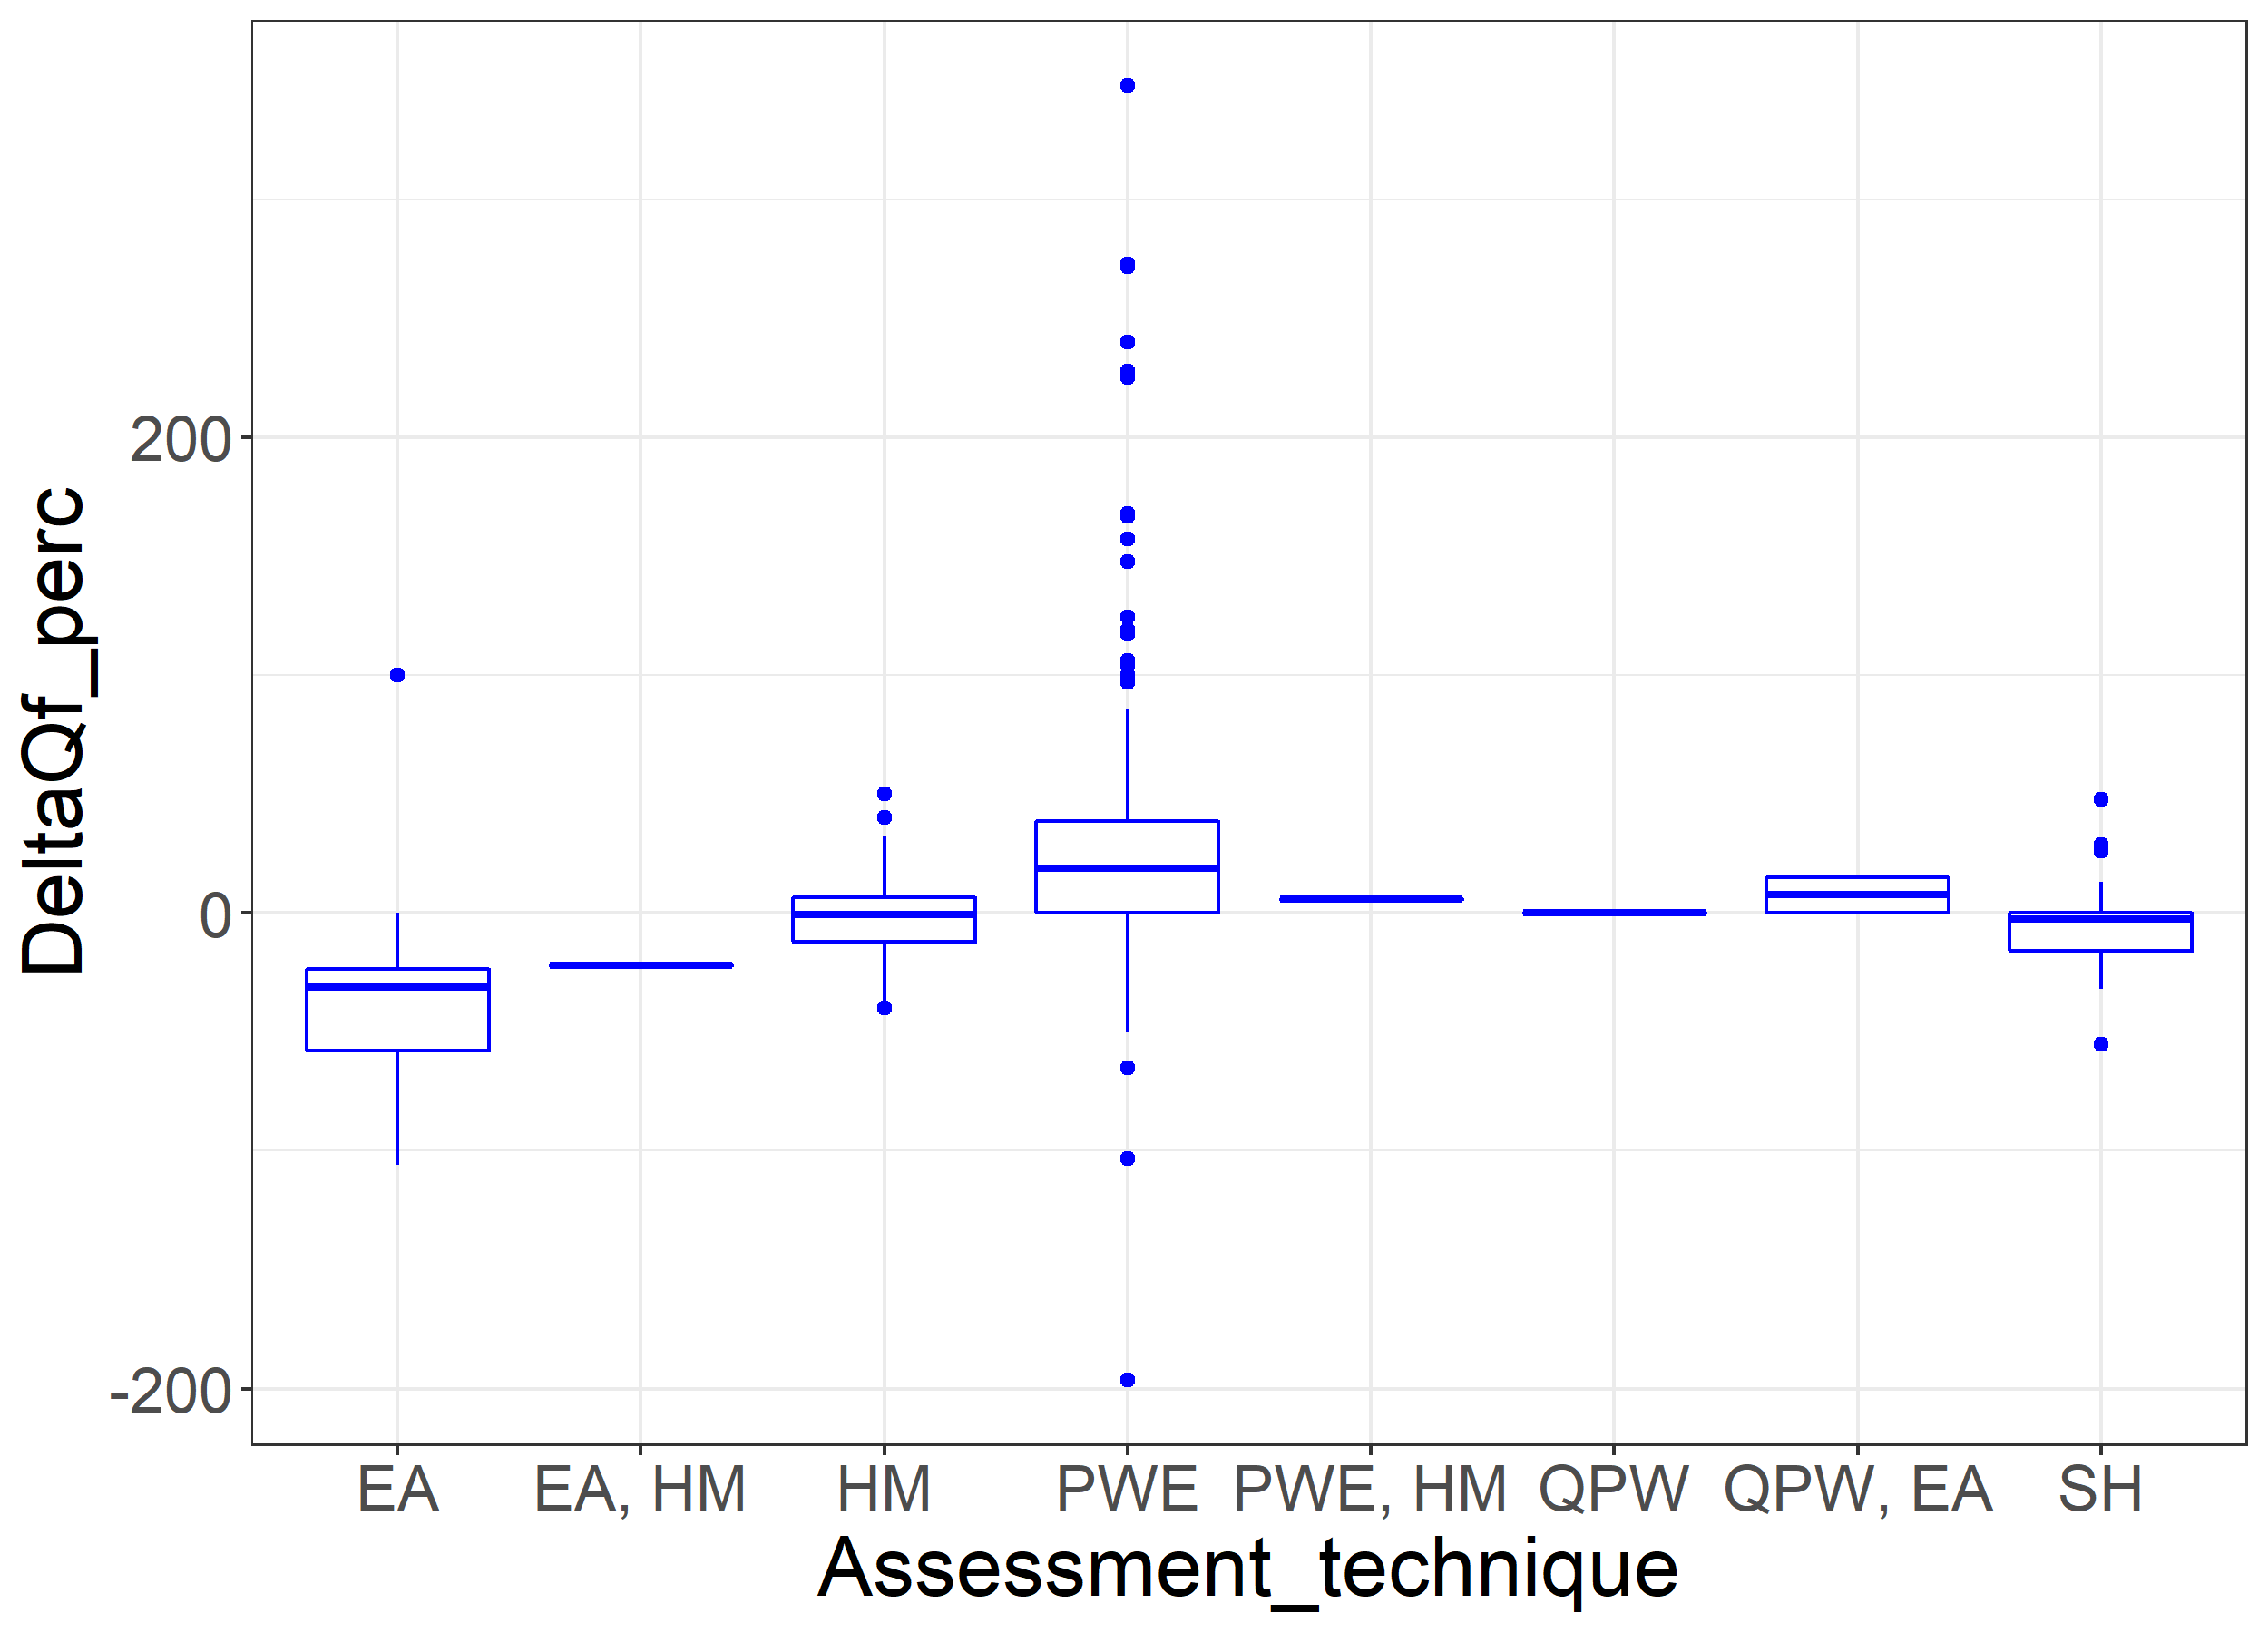
\includegraphics[width=0.9\linewidth]{AssessmentTechnique_byDeltaQf} \caption{Boxplot of the variation in the change in flow for the different assessment techniques, showing the dominance of the variation and the outliers in the dataset in the paired watershed experiments}\label{fig:assessment}
\end{figure}

\hypertarget{general-discussion}{%
\subsection{General discussion}\label{general-discussion}}

In this paper, a few studies have been singled out to demonstrate the main point that extrapolating individual studies to global scales is not that simple in natural systems. Not only is there significant natural variation and latent variables, interpretation and aggregation can cause further unforeseen problems. The choice of papers to focus on was mainly driven by the data that was made available by the authors of these papers \citep{zhang2017, filoso2017}, which provide a rich case study for the current paper.

Field research is by nature limited in space and time, due to the high costs involved of setting up experiments. This is particularly true for experiments in hydrology and forest hydrology, where field sites need to cover sufficient spatial and temporal variability. This means there is a general need to extrapolate the local results to larger scales to inform decision making and policy.

However, as is demonstrated in this paper, there are multiple issues when this local scale data is extrapolated to larger scales. It clearly demonstrates that the results of any model (in this case a regression model) is highly dependent on the data, but also on the assumptions in the model. From the perspective of extrapolating local data to global scales for policy advice and decision making \citep[i.e.][]{hoekvandijke2022, jackson2005}, this is an important point.

\hypertarget{residuals-of-the-model}{%
\subsubsection{Residuals of the model}\label{residuals-of-the-model}}

The residuals of the final model presented in this paper (Figure \ref{fig:gamcheckmodelall}) indicate that the residual distribution remains fat-tailed, causing deviations from an assumed \(\epsilon \sim N(0,\sigma^2)\). This once again highlights that there is unexplained variation at the extremes of the distribution, once again related to the paired watershed experiments (Figure \ref{fig:assessment}). Generally,in statistical models, the approach would be to further normalize the residuals through transformations. However, in this case this might be difficult and might not resolve all the issues due to the large variation in the data.

\hypertarget{interactions}{%
\subsubsection{Interactions}\label{interactions}}

The current modelling approach does not consider any interactions between the variables, and this would offer another approach to understand the variation in the data. As already indicated in Figure \ref{fig:corgraphs}, there are interactions between different variables. This further complicates the extrapolation of the local scale experiment data to global scales and to extend historical data to current management and decisions.

In this case, interactions were not included because, as was shown, there are bigger problems with trying to extrapolate the existing data, and the data itself can be problematic. To be able to model the interactions well, the nature of the variables and interactions need to be understood and or clearly hypothesized. Otherwise it becomes another case of correlation without causation.

\hypertarget{implications-for-other-meta-analysis-studies}{%
\subsubsection{Implications for other ``meta-analysis'' studies}\label{implications-for-other-meta-analysis-studies}}

There has been a recent push to develop more meta-analysis studies in hydrology \citep{wang2020, evaristo2020metaanalysis}, and we strongly believe that developing new insights by combining historical data sets from reviewed papers is highly valuable. However, this paper highlights that there is considerable chance that large historical data sets include latent variables and are more complex than envisioned. This is particularly true for work in natural systems and more historical work, as methods of observation and even approaches to management have changed considerably. The same management description is not necessarily the same action on the ground. A carefully designed and systematic approach can prevent some of bigger problems as is demonstrated in \citet{wang2020}, where both the approach and the catchment area are investigated as latent variables.
This is particularly relevant, where the results of meta-analyses are extrapolated to make global predictions without clearly quantified uncertainties (such as in \citet{hoekvandijke2022} and \citet{wang2020}).

A second potential danger is the extrapolation of the local small catchment results and conclusions to larger scales, but beyond the original scope of the studies. For example, the current database is mainly related to forest harvest, bush fire and reforestation/plantation management. It is tempting to use the result of a large scale analysis of this data to make inferences about overall land use change \citep{li2017, wang2020}, but this would not be valid, as not all deforestation studies are a transition to an agricultural land use or pasture, as in \citet{levy2018}. Many are logging or bushfire studies regrowing into forest after the initial treatment. Similarly, using the plantation studies to extrapolate to ``reforestation'' (as in \citet{filoso2017} and \citet{hoekvandijke2022}) is also tenuous. Plantation forests are generally fast growing hybrids that will have quite different ecophysiology, particularly in South America \citep{jones2017, binkley2017}, while other reforestation, for example for salinity control in Australia, might focus on a mix of native species. Given the link between ecophysiology and water and carbon budgets \citep{jackson2005}, care should be taken in extrapolation, introducing a further error.

As highlighted summarizing highly variable observed time series into single mean values introduces further potential problems, as well as discarding information about the variance.

A final factor is ignoring the effect of climate change \citep{vervoort2021} on runoff, even if the effects are still minor. Earlier papers \citep{li2017, wang2020} have analyzed climate effects relative to management effects in the data, but these studies did not explicitly test for climate change. Given that the database of studies now captures almost 100 years of work, we cannot ignore a climate change trend that is potentially hidden in the data. A simple inclusion of the start date of the experiment (\emph{From}) in the GAM model does suggests an increase in change in the percentage of flow over time. However, as the data distribution is uneven in time, and consists of multiple assessment techniques there could be multiple complicating factors, and drawing a firm conclusion would be premature.

\hypertarget{future-research-needs-implications-for-forest-hydrology}{%
\subsubsection{Future research needs (implications for forest hydrology)}\label{future-research-needs-implications-for-forest-hydrology}}

Beyond a more formal approach to investigating climate change effects in the data, this study also points to several further opportunities and future research needs.

A major focus of many of the papers related to forest hydrology has been on the impact of plantation forest operations on the catchment, rather than the transition of forestry to agriculture. As the paper by \citet{jones2017} highlights this means there are opportunities to analyze the time evolution of the catchment response to forestation. Given the large number of studies that look at a time evolution of forest cover (i.e.~either clearing and regrowth, or burning and regrowth), this data can offer further insights into the dynamic response of catchments to changes in land cover. In addition, this might allow analysis of the variance of the response in addition to the mean response. While some of the older data is not fully recoverable, but there is often a series of papers related to one experiment, which at least would provide individual time points.

More generally there is a clear need for a more in depth analysis of the data base of studies used here. In particular, more detailed data can potentially be extracted from many of the studies in terms of vegetation species, stream flow responses and responses of components of stream flow (slow flow, quick flow etc.), as well as a more in depth description of the management and actual experimental design.

There is also a clear need to understand the impact of the assessment methods with respect to scale. Extrapolating paired watershed experiment results into models can possibly overlook landscape interactions that are visible at larger scales, but do not occur on smaller scales. For example, this could be the effects of lateral flow and groundwater connectivity and impacts of elevation on land use. A carefully designed simulation study that specifically investigates the change in stream flow response with scale using local field data for verification can help solve this problem.

At the moment, providing answers to the impact of stream flow at larger scales should generally not be approached by simulation modelling. A better approach is analyzing stream flow data at multiple spatial and temporal scales for responses (rather than running simulations) and using satellite data to dynamically include land use changes. The highlighted paper by \citet{levy2018} is currently the best example of a solid statistical approach to analyzing stream flow responses. Simulation modelling can be an approach to analyze different scenarios, if there is clear recognition of the potential impact of the model structure (the algorithms and parameters that describe for example plantation tree growth) on the simulation outcomes.

We envision that in the future more innovative approaches to analyzing data at different scales will be developed.

\hypertarget{conclusions}{%
\section{Conclusions}\label{conclusions}}

This study demonstrates that the analysis of large databases of essentially ``aggregated data'' should be considered carefully and simple single variable regressions often present simplistic relationships that can be misleading.

On first glance, stream flow will decrease with increases in forest cover, and increase with removal of forest cover. However, the conclusions on the exact relationship between stream flow change and forest cover change are highly uncertain. There are four major interlinked reasons why earlier conclusions should be considered carefully:

\begin{itemize}
\tightlist
\item
  The existence of latent variables in the data that create the appearance of a relationship that really does not exist. In this case the assessment technique used to assess the change in stream flow is highly significant;\\
\item
  The difficulty in fully interpreting the specifics of different studies. In this case the definition of vegetation, stream flow volume, control or time period was difficult to assess;\\
\item
  The difficulty of integrating data from seemingly similar studies, but with quite different objectives. This study highlighted the many logging studies followed by regrowth, or bushfire effects; and\\
\item
  The chance of transcription errors influencing the data.
\end{itemize}

While some of these issues might be overcome with careful analysis and transcription, not all can be directly or easily resolved. Any statistical analysis, including the one in this paper, needs to be considered ``conditional on the data'', and given the issues indicated, extrapolation of the results of summary studies to larger scales and into global hydrological models has to be done with great care. Better would be to analyze observed data and explicitly include uncertainty in the extrapolation of the results. This therefore has implications for the recent growth in meta-analysis review papers, which has been boosted by increased computational capacity and much better on-line accessible data bases with research data. This is particularly true for natural systems involving climate variability and therefore extrapolations of experimental work in Environmental Science and Hydrology to global scales in general.

\hypertarget{acknowledgements}{%
\section{Acknowledgements}\label{acknowledgements}}

This work was funded through project FPTA 358, Instituto Nacional de Investigacion Agropecuaria, INIA-Uruguay.

\hypertarget{credit-statement}{%
\section{CRediT Statement}\label{credit-statement}}

R. Willem Vervoort: Conceptualization, Methodology, Code, Writing- Original draft preparation, Writing- Reviewing and Editing. Eliana Nervi: Data curation, Writing- Original draft preparation, Writing- Reviewing and Editing. Jimena Alonso: Conceptualization, Writing- Reviewing and Editing.

\renewcommand\refname{References}
\bibliography{forestandwater.bib}


\end{document}
